\documentclass[12pt]{article}

\usepackage[english]{babel}
\usepackage[utf8]{inputenc}
\usepackage{amsmath,amssymb}
\usepackage{parskip}
\usepackage{graphicx}
\usepackage{multicol}
\usepackage{float}


% Margins
\usepackage[top=1.5cm, left=2cm, right=2cm, bottom=2.0cm]{geometry}
% Colour table cells
\usepackage[table]{xcolor}

% Get larger line spacing in table
\newcommand{\tablespace}{\\[1.25mm]}
\newcommand\Tstrut{\rule{0pt}{2.6ex}}         % = `top' strut
\newcommand\tstrut{\rule{0pt}{2.0ex}}         % = `top' strut
\newcommand\Bstrut{\rule[-0.9ex]{0pt}{0pt}}   % = `bottom' strut

%%%%%%%%%%%%%%%%%
%     Title     %
%%%%%%%%%%%%%%%%%
\title{Synthèse Artificial Inteligence LINFO1115}
\author{Jacques HOGGE}
\date{\today}

\begin{document}
\maketitle
\newpage
\tableofcontents
\newpage

%Introduction
\section{Introduction}

	Plusieur def pour IA, pas encore acceptées
	
	C'est un "Umbrella Terme" (représente in concept), c'est multidisciplinaire car souvent modifié.
	
	\begin{figure}[H]
		\centering
		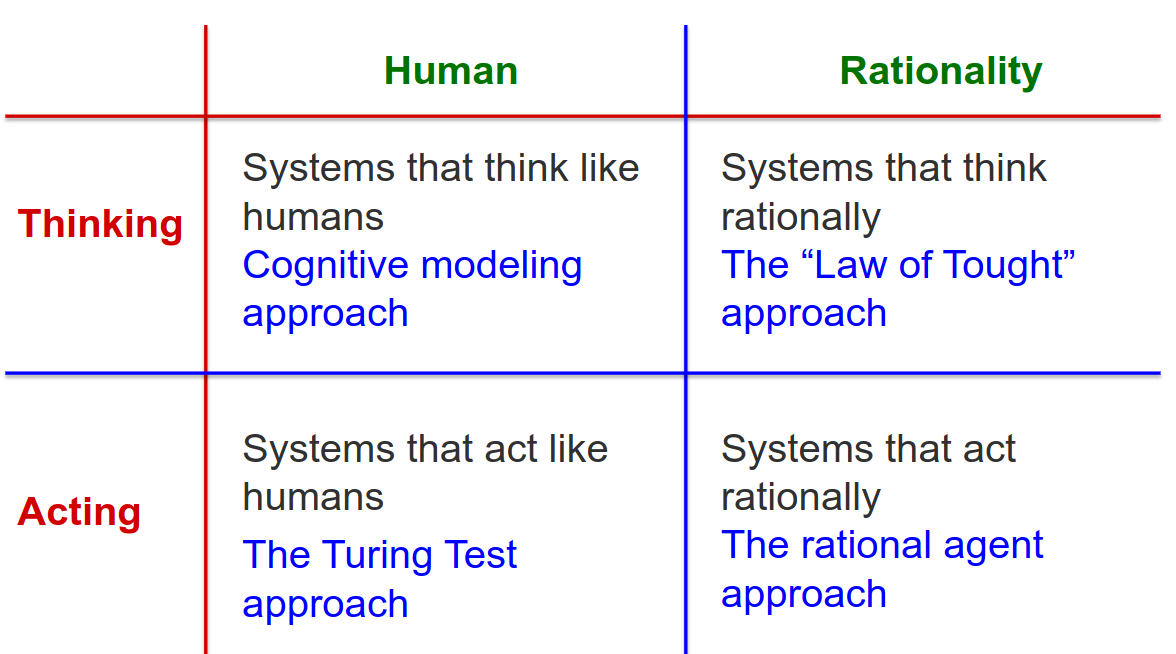
\includegraphics[width=\textwidth]{img/IA.png}
	\end{figure}
	Une intelligence artificielle est est système qui peut :
	\begin{itemize}
		\item penser comme un humain ?
		\item agir comme un humain ?
		\item \dots 
	\end{itemize}
	\subsection{Turing test}
		une IA est "réussie" si un humain pense que il parle avec un humain

\newpage

%2.1-2.3
\section{2.1-2.3}
\subsection{Agents and environnements}
	\begin{figure}[H]
		\centering
		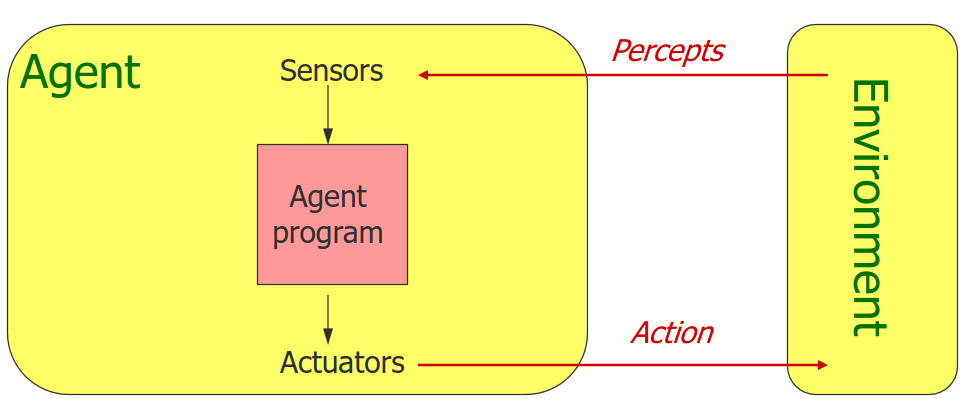
\includegraphics[width=\textwidth]{img/agent.png}
		\caption{Agent}
	\end{figure}
	
	\begin{itemize}
		\item \textbf{Agent} : Entité qui interagi avec son environnement, perception avec des sensors et action avec des actuators
		\item \textbf{Percept} : Perception de l'agent a un instant $t$
		\item \textbf{Percept sequence} : Historique complet des percept d'un agent
	\end{itemize}
\subsection{Concept of Rationality}

	\textbf{Rationalité} : " Faire la bonne action ", l'action qui amène au meilleur résultat. Mais un ordinateur ne sais pas c'est quoi la bonne chose a faire. On va donc avoir besoin d'une \textbf{Performance measure} qui va calculer un score si l'action est bonne ou pas.
	
	\textbf{Agent rationnel} : Pour chaque séquence d'action possible, un agent rationnel doit sélectionner un action qui maximise la \textbf{Performance measure}.
	
	La rationalité d'un action dépend de :
	\begin{enumerate}
		\item Une \textbf{Performance measure} qui dépend des critères de succès
		\item La connaissance préalable de l'environnement par l'agent
		\item Les actions que l'agent peut faire
		\item La séquence de perception actuelle de l'agent
		
	\end{enumerate}
	
	Attention, \textbf{Rationality $\neq$ Omniscience}
	
	\textbf{Agent omniscient} : sait le réel résultat de ses actions
	
	\textbf{Agent autonome} : apprend ce qu'il peut faire pour compenser ce qu'il ne sait pas faire. (machine learning)
	
\subsection{Nature et environnements}
	Environnement de travail d'un agent est spécifique a (PEAS) \textbf{P}erformance, \textbf{E}vironnement, \textbf{A}ctuators, \textbf{S}ensors.
	
	\begin{figure}[H]
		\centering
		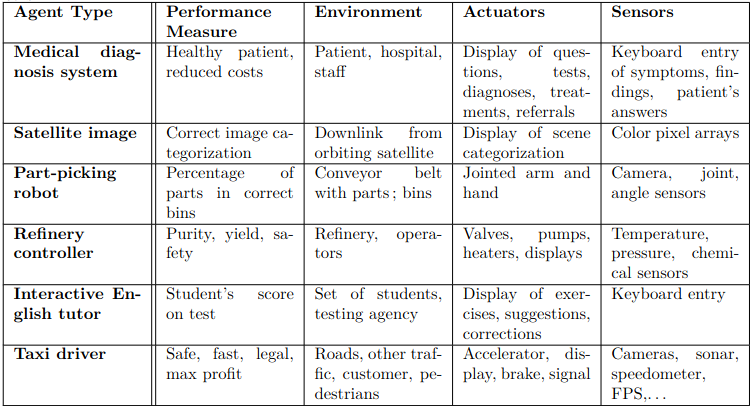
\includegraphics[width=\textwidth]{img/PEASexemple.png}
		\caption{Exemple PEAS}
	\end{figure}	
	
	Les propriété sont les suivante:
	
	\textbf{Fully observable vs. Partially observable} : Toutes les informations pertinentes sont accessibles (échecs vs poker)
	
	\textbf{Single agent vs. Multiagent} : il y a t'il plus que 1 agent, si oui c'est une compétition ou coopération ? (crossword puzzle vs chess)
	
	\textbf{Deterministic vs. Stochastic} : (Chess vs.Poker)
	\begin{itemize}
		\item Le prochain état (state) de l'environnement dépend entièrement de l'action de l'agent.
		\item L'environnement pour l'agent est moins déterministe car il ne dispose pas de toutes les informations sur l'environnement.(Il ne peut pas déterminer avec précision l'état suivant à cause du hasard).
	\end{itemize}
	\textbf{Episodic vs. Sequential} : L'expérience de l'agent est divisée en épisodes atomiques indépendants les uns des autres.
	
	\textbf{Static vs. Dynamic} : L'environnement peut changer quand l'agent est entrain de réfléchir.
	
	\textbf{Discrete vs. Continuous} : Le nombre différent de state est fini et l'ensemble des actions est discret (chess vs. taxi driving)
	
	\textbf{Known vs. Unknown} : le résultat de chaque action est donné. Ce n'est pas la même chose que d'être totalement observable, par exemple les jeux vidéo, on connaît toutes les informations via l'écran mais on ne sait pas ce que fait le bouton.
	
	\begin{figure}[H]
		\centering
		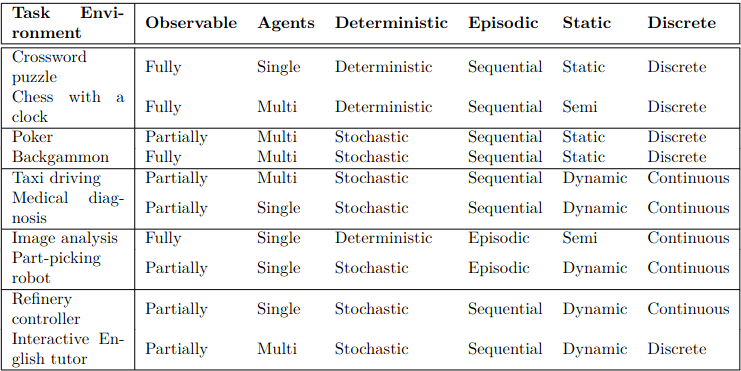
\includegraphics[width=\textwidth]{img/PEASexemple2.png}
	\end{figure}

\newpage

%Solving Problem by searching
\section{ Solving probleme by search}
\subsection{Structure d'un agent}
	Un agent est composé de 2 partie :
	\begin{itemize}
		\item \textbf{Architecture} : c'est les composants de l'ordinateur sur le quelle l'agent tourne
		\item \textbf{Programme} : Se sont les fonctions qui Map les perceptions en actions
	\end{itemize}
	
	Exemple d'un programme d'agent:
	
	\begin{itemize}
		\item Table de conduite de l'agent (\textbf{table driven})\\
		\item \textbf{Successor} : Tous les states atteignable depuis le state actuelle\\
		\item \textbf{Path} : Séquence de states connecté par une sequence d'action\\
		\item \textbf{Operators} : Manière de modifier un state avec une action\\
		\item \textbf{Goals Test} : Fonction qui teste si un state est le résultat final\\
		\item \textbf{Step Cost} : Cout numérique de passer du state $s$ avec l'action $a$ pour passer au state $s'$\\
		\item \textbf{Path Cost} : Fonction qui donne un cout a chaque path\\
		\item \textbf{Solution} : Séquence d'action de l'initial state jusqu'au goal state\\
		\item \textbf{Optimal Solution} : Solution avec le path avec le plus petit cout parmi toutes les solutions\\
		\item \textbf{Node} : Data structure qui constitue les graph et arbre de recherche\\
		\item \textbf{Frontier} : Ensemble de Node généré au quelle les ancêtre on été Goal-tested (visited)\\
		
		\item \textit{C'étais long mais bon fallait le faire}
		
	\end{itemize}
	\subsection{Problem solving Agent}
		\subsubsection{Definition Probleme}
			Un problème peut être définie avec :
			\begin{enumerate}
				\item States ou Initial State
				\item Une description des actions possible et valide par l'agent
				\item Une description de quoi chaque action fait (transition model)
				\item Un Goal test
				\item Un Path cost qui utilise un step cost
			\end{enumerate}
		\subsubsection{Solution}
			Une solution est une séquence d'action qui commence du state initial et qui termine à un des goal state. La solution est optimal si elle a la plus petite path cost parmis toutes les solutions
		\subsubsection{State space}
			Ensemble qui représente le problème avec les actions, les couts, ... (graph représentation). Possibilité d'un ensemble infini de states.
			\begin{figure}[htp]
				\centering
				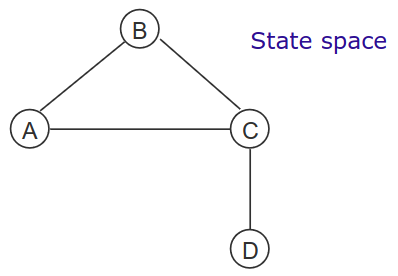
\includegraphics[width=.5\textwidth]{img/StateSpace.png}
			\end{figure}
		\subsubsection{Search Tree}
			Représentation du problème sous la forme d'arbre, avec les path entre les states et les goals. multiple path. Et un seul path d'un node a la racine.
			\begin{figure}[htp]
				\centering
				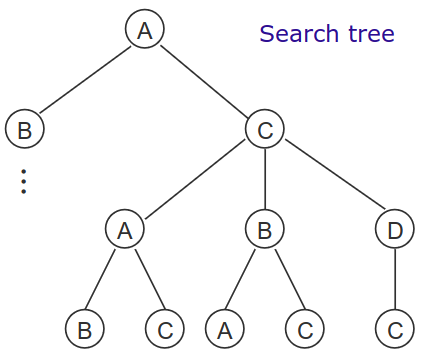
\includegraphics[width=.5\textwidth]{img/SearchTree.png}
			\end{figure}
			
		\subsubsection{State and Nodes}
			\begin{itemize}
				\item \textbf{State} représentation d'un configuration physique qui represente un state intermédiaire.
				\item \textbf{Node} data structure qui constitue le search tree
			\end{itemize}
			il peut y avoir plusieurs nodes avec le même state
		\subsubsection{Repeated States}
			On va éviter de visiter des Nodes qui on déjà été visité avant, pour cela, on va utiliser la représentation en arbre (search tree) et on ne pas va \textit{Expand} les nodes déjà visité.
	\subsection{Searching for Solutions}
		Trouver une solution est le fait de traverser un state space (graph ou tree) et du initial state au goal state avec un ensemble d'actions valide.


		\textbf{Expanding} : appliquer chaque action légal au state actuel.
		\begin{figure}[htp]
			\centering
			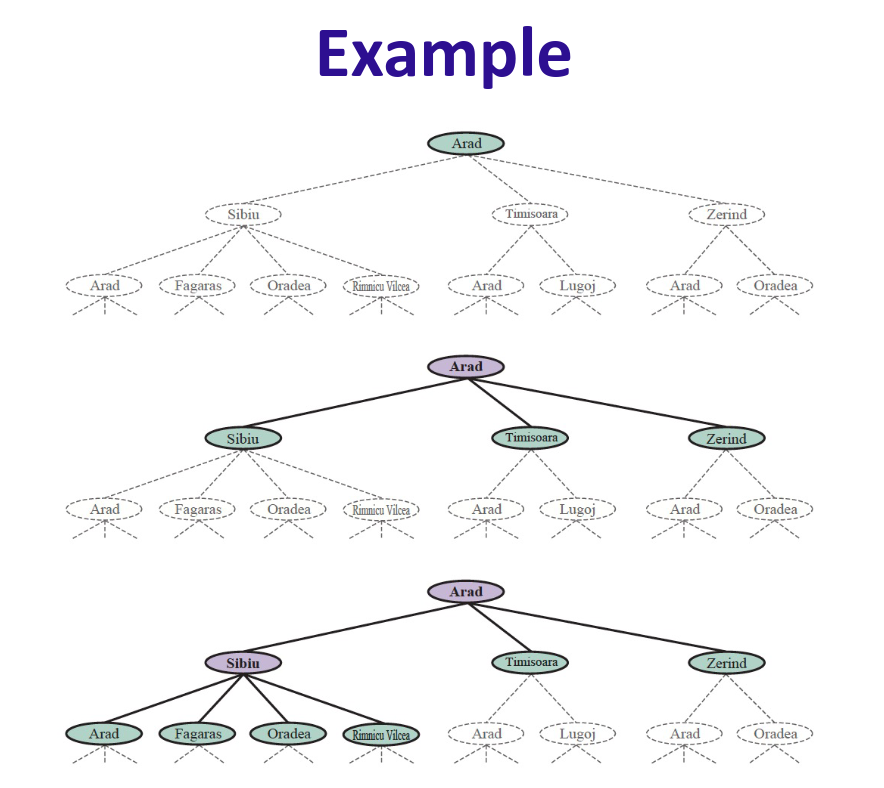
\includegraphics[width=0.6\textwidth]{img/ExempleExpanding.png}
		\end{figure}
		
		\textbf{Frontier} : Ensemble des node non-Expanded au quelle les ancêtres on déjà été visité. La frontière peut être représenté grâce a une Data structure Queue (lol zizi), On peut utiliser un Priority, LIFO, FIFO, \dots
		\begin{figure}[htp]
			\centering
			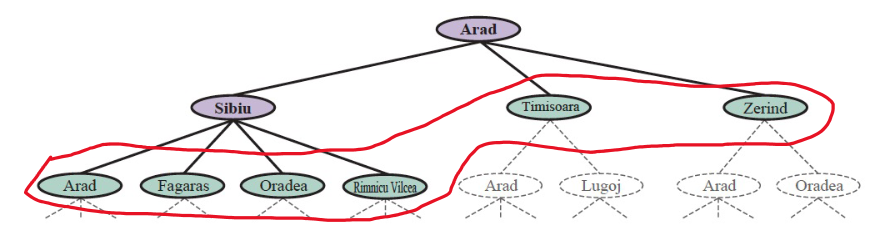
\includegraphics[width=0.6\textwidth]{img/FrontierExemple.png}
		\end{figure}
		
		\subsubsection{Stratégies}
			Il y a 2 types de recherches: 
			\begin{enumerate}
				\item \textbf{uninformed search} où la seul information de l'agent est \textit{"suis-je le but final ?"}.
				\item \textbf{informed search} où l'agent a les informations d'avant.
			\end{enumerate}
			
			On peut évaluer ces recherche avec 4 critères:
			\begin{itemize}
				\item \textbf{Completeness} : l'agent trouve un solution s'il en existe au moins une.
				\item \textbf{Time complexity} : Souvent en terme du nombre de nodes généré/Expanded
				\item \textbf{Space complexity} : Nombre de node en mémoire
				\item \textbf{Optimality} : Trouve solution avec le cout minimal 
			\end{itemize}
			
			On va utiliser 3 variables :
			\begin{itemize}
				\item \textbf{b} : Facteur de branchement maximal du Search tree
				\item \textbf{d} : Profondeur de la solution la moins couteuse
				\item \textbf{m} : Profondeur max de l'arbre (peut etre $\infty$)
			\end{itemize}
			
			\begin{figure}[H]
				\centering
				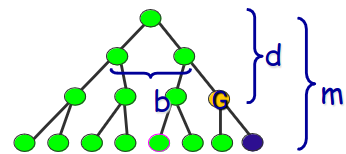
\includegraphics[width=.5\textwidth]{img/BDM.png}
			\end{figure}
	\subsection{Uninformed Search}
		\begin{figure}[htp]
			\centering
			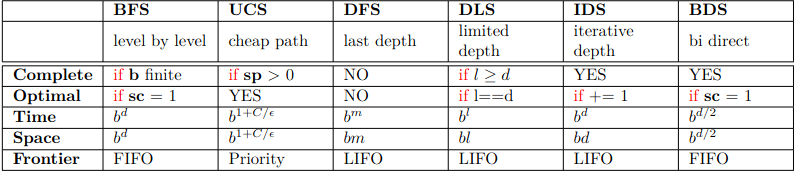
\includegraphics[width=\textwidth]{img/UninformedSearch.png}
		\end{figure}
		\subsubsection{Breadth-First Search(BFS)}
			Le but est de vérifier par niveau de l'arbre. Problème la mémoire est vite remplie. On commence du root node et ensuite on passe au sub-nodes qui sont dans une FIFO Queue qui représente la frontière.
			
			\begin{itemize}
				\item \textbf{Complétude} : Oui
				\item \textbf{Complexité temporelle} : $\mathcal{O}(b^d)$\footnote{$1+b+b^2 + \dots + b^d$}
				\item \textbf{Complexité spatiale} : $\mathcal{O}(b^d)$
				\item \textbf{Optimal} : Oui si cout = 1 (pas souvent le cas)
			\end{itemize}
			
			\begin{figure}[htp]
				\centering
				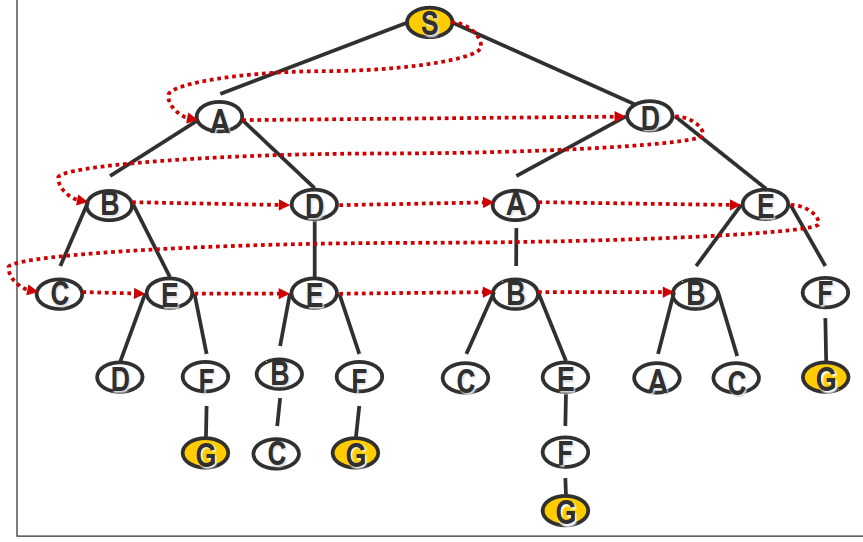
\includegraphics[width=0.6\textwidth]{img/BFS.png}
				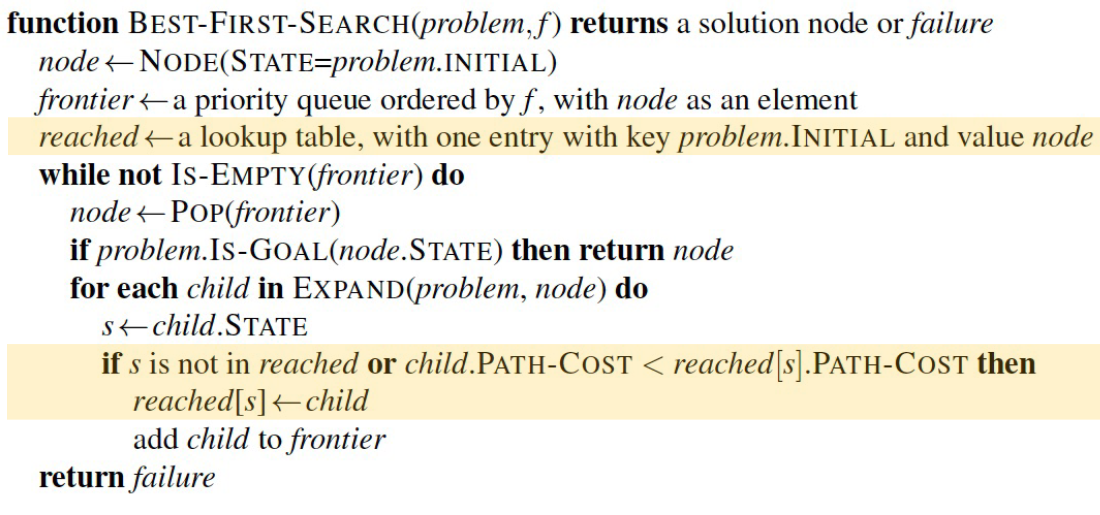
\includegraphics[width=\textwidth]{img/CodeBFS.png}
			\end{figure}					
		\newpage
		\subsubsection{Uniform-Cost search (UCS)}
			Comme le BFS sauf que le Node avec le cout le plus petit est exploré en premier. Il y a un cout pour passer d'un node a l'autre. La frontière est implémenté avec un Priorety Queue. Fort semblable a Dijkstra.
			
			\begin{figure}[htp]
				\centering
				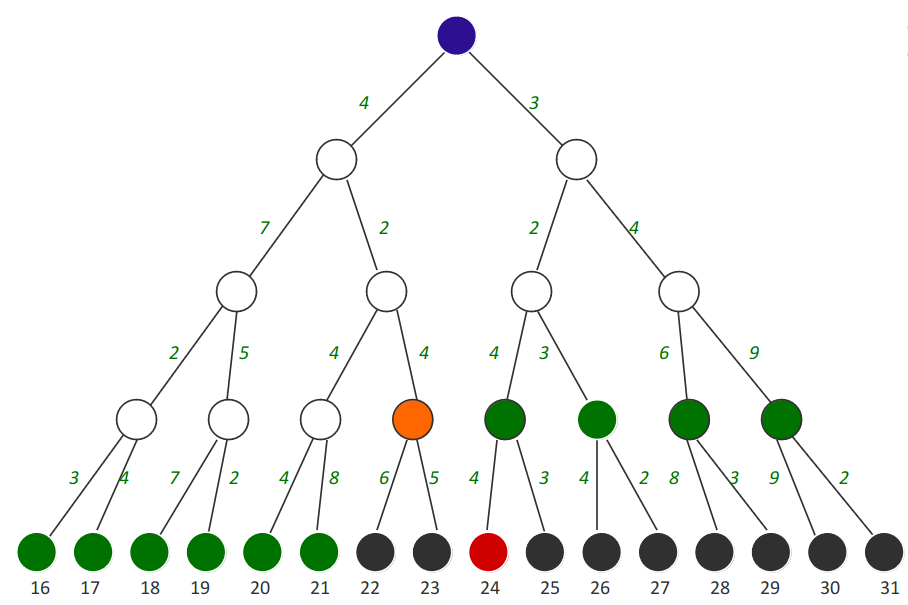
\includegraphics[width=0.6\textwidth]{img/UCS.png}
			\end{figure}
			
			\begin{itemize}
				\item \textbf{Completude} : Si cout strictement positif ($\geq \epsilon \geq 0$)
				\item \textbf{Complexité temporelle} : Dure a dire
				\item \textbf{Compelxité spatiale} : $\mathcal{O}(b^{C^{*/\epsilon}}$
				\item \textbf{Optimal} : Oui
			\end{itemize}
			
			
			
		\subsubsection{Depth-first Search (DFS)}
		Concrètement, on visite toutes une branche de l'arbre jusqu'à arriver à la \textit{Leaf}, si on ne trouve pas le goal on passe a la prochaine, etc.
		La Frontière est implémenté avec un Queue LIFO.
		
		\begin{itemize}
			\item \textbf{Complétude} : Non car peut avoir profondeur (m) $\infty$
			\item \textbf{Complexité temporelle} : $\mathcal{O}(b^m)$ mauvais si ($m > d$)
			\item \textbf{Complexité spatiale} : $\mathcal{O}(mb)$
			\item \textit{Optimal} : Non
		\end{itemize}
		
		\begin{figure}[htp]
			\centering
			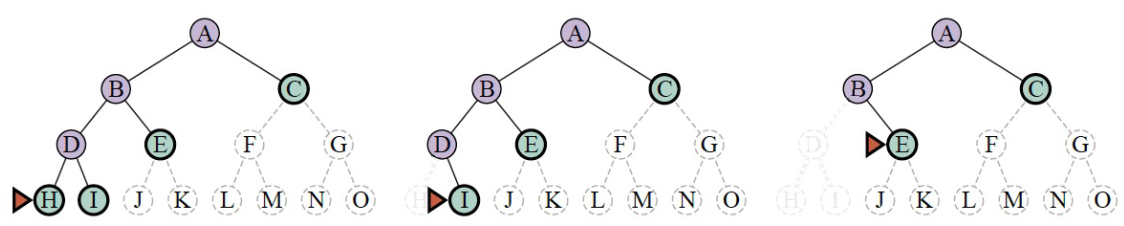
\includegraphics[width=\textwidth]{img/ExempleDFS.png}
		\end{figure}
		
		\subsubsection{Depth-Limited Search}
			Pareil de DFS sauf que la on met une limite de profondeur(depth) $l$.
		
		\subsubsection{Iterative Deepening}		
		  Pareil que DLS mais si $l < d$ alors on ne trouveras jamais de solutions, donc on va incrémenter petit a petit $l$
			\begin{figure}[htp]
				\centering
				$l = 1$
				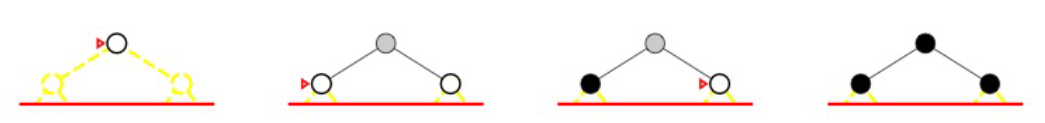
\includegraphics[width=\textwidth]{img/DLS1.png}
				$l = 2$
				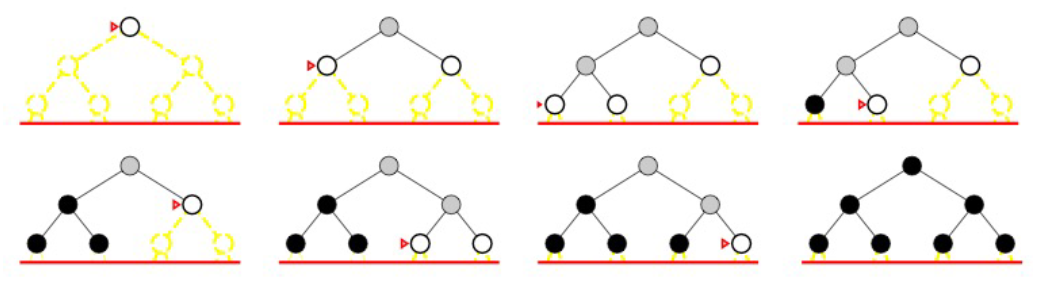
\includegraphics[width=\textwidth]{img/DLS2.png}
				$l = 3$
				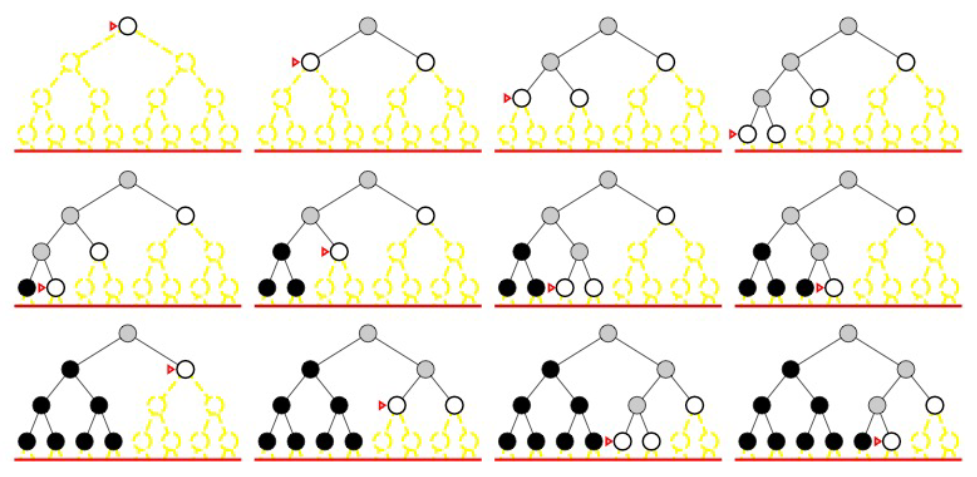
\includegraphics[width=\textwidth]{img/DLS3.png}

			\end{figure}
			
		Plusieurs nodes sont visité plusieurs fois, mais ce n'est pas très grave car il n'y en a pas beaucoup.
		
		\begin{itemize}
			\item \textbf{Complétude} : Oui
			\item \textbf{Complexité temporelle} : $\mathcal{O}(b^d)$
			\item \textbf{Complexité spatiale} : $\mathcal{O}(b^d)$
			\item \textbf{Complétude} : Oui si cout = 1
		\end{itemize}
		
		
		\subsubsection{Biderectional Search}
			On commence du root jusqu'au Goal et aussi du Goal jusqu'au root et on stoppe quand les 2 s'intersecte. Il y quelque difficulté.
			\begin{itemize}
				\item Prédécesseurs du goal doivent être généré (pas toujours possible)
				\item Search doit être coordonnée entre les 2 recherches
				\item Problème si plusieurs Goal
				\item Tous les nodes doivent rester en mémoire
			\end{itemize}
			
			\begin{itemize}
				\item \textbf{Complétude} : Oui
				\item \textbf{Complexité temporelle} : $\mathcal{O}(b^{d/2})$
				\item \textbf{Complexité spatiale} : $\mathcal{O}(b^{d/2})$
				\item \textbf{Optimal} : Oui si cout = 1
			\end{itemize}
			
	\subsection{Informed Search}
		En utilisant des connaissances spécifiques au problème, trouver et/ou déduire des informations sur les States futurs et les paths futures.
		
		BFS est un algo de recherche ou les nodes sont sélectionner pour êtres \textit{Expand} basé sur \textbf{une fonction d'évaluation} $f(n)$, cela donne un cout et on choisi le node avec le plus petit cout avec une Priority Queue.
		
		Attention on calcule une évaluation et non pas la distance exacte
		
		\subsubsection{Heuristic Fonction}
		
		Noté $h(n)$ est une fonction qui estime le cout d'un node vers le goal. c'est une approximation car on ne connait pas le cout exacte.
		\begin{figure}[htp]
			\centering
			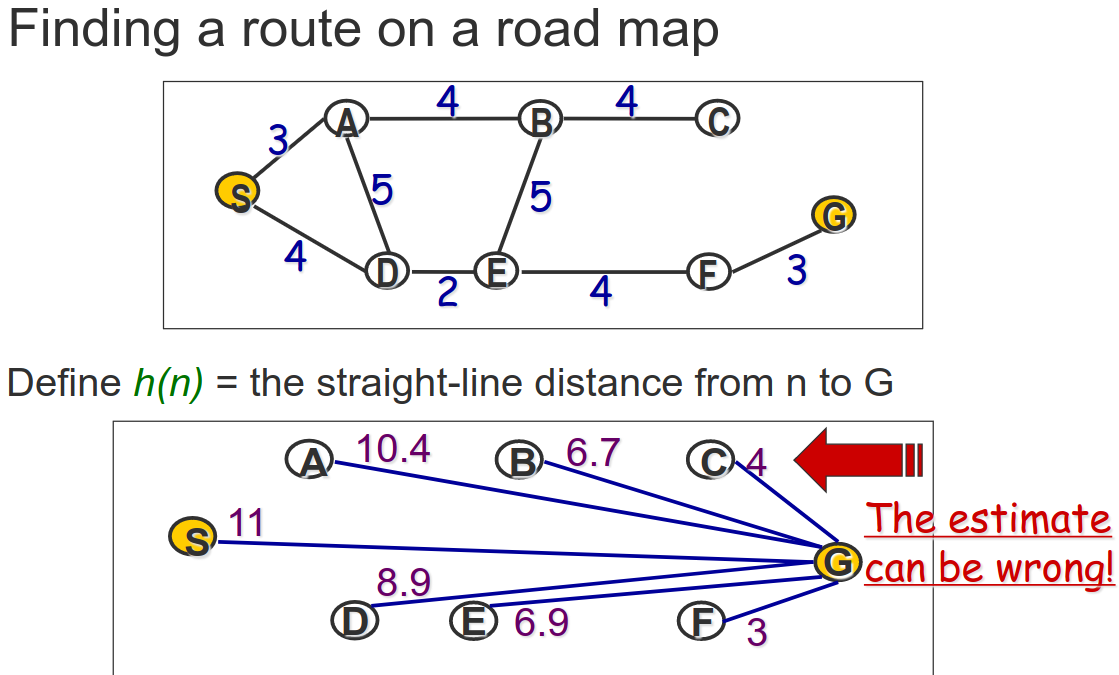
\includegraphics[width=0.8\textwidth]{img/ExempleHeuristic.png}

		\end{figure}
		
		Il y a 3 types de fonction Heuristique :
		\begin{itemize}
			\item \textbf{Optimistic} : Admissible car elle pense que le cout pour résoudre le problème est inférieur au cout réel
			\item \textbf{Admissible} : Ne surestime jamais le cout pour atteindre le goal. Le cout qu'il estime est plus grand que le plus petit cout possible par rapport au node actuel. $h(n) = 0$ si c'est un Goal state.
			\item \textbf{Consistent} : L'estimation de un node $n$ au goal est plus petit que le cout réel de $n$ a un nouveau node $n'$ avec l'action $a$ plus l'estimation de $n'$ au goal 
			\begin{equation}
				h(n) \leq c(n,a,n') + h(n')
			\end{equation}
		\end{itemize}
		
		un consistent heuristi est admissible
		
		\subsubsection{Triangle inequality}
			\begin{figure}[htp]
				\centering
				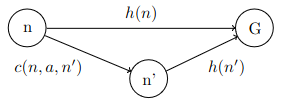
\includegraphics[scale=1]{img/Triangle.png}
			\end{figure}
			Chaque coté du triangle ne peut pas être plus long que la somme des autres cotés.
			\begin{itemize}
				\item \textbf{h(n)} : Estime le cout entre $n$ et $G$
				\item \textbf{C(n,a,n')} : cout pour aller en $n'$ depuis $n$ avec l'action $a$
				\item \textbf{h(n')} : cout estimé entre $n'$ et $G$
			\end{itemize}
			
		\subsubsection{Monotonicity} 
			Si $h(n)$ est consistant alors f(n) le long d'un path quelconque n'est pas décroissant. Supposons que $n'$ est un successeur de $n$ alors :
			
			\begin{figure}[htp]
				\centering
				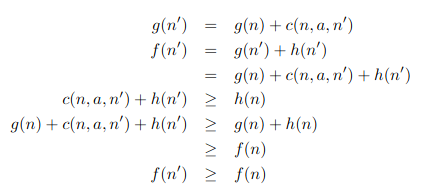
\includegraphics[scale=1]{img/Monotonicité.png}
			\end{figure}
		\subsubsection{Greedy Best-First Search(GBFS)}
			Tente d'étendre le node qui est le plus proche du Goal. Donc ici, $f(n) = h(n)$
						
			\begin{itemize}
				\item \textbf{Complétude} : Non, profondeur peut etre infinie
				\item \textbf{Complexité temporelle} : $\mathcal{O}(b^m)$
				\item \textbf{Complexité spatiale} : $\mathcal{O}(b^m)$
				\item \textbf{Optimal} : Non
			\end{itemize}
			
			\begin{figure}[htp]
				\centering
				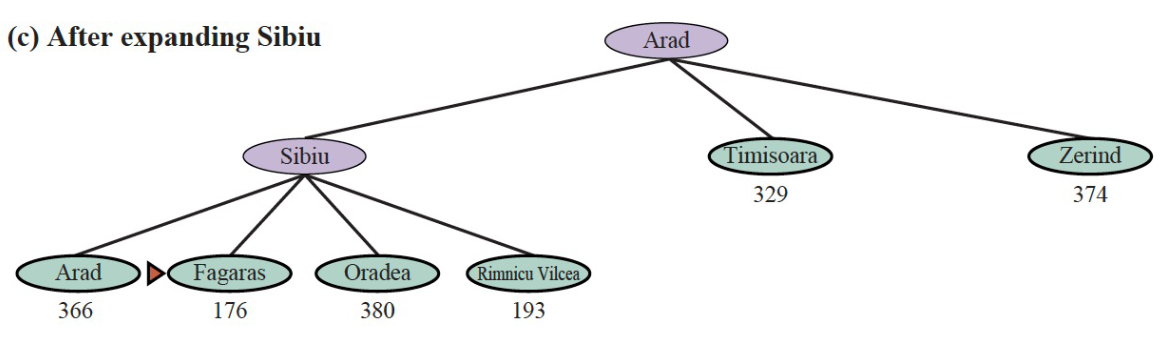
\includegraphics[width=\textwidth]{img/GBFS.png}
			\end{figure}
			
		\subsubsection{A*}
		Fusion de GBFS et Uniform cost. Minimise le cout total estimé de la solution
		
		\begin{figure}[H]
			\centering
			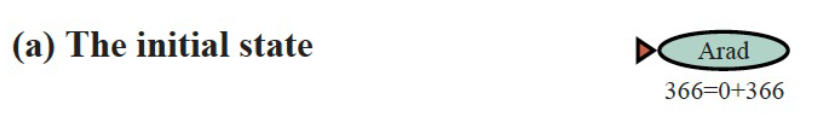
\includegraphics[width=\textwidth]{img/A.png}
		\end{figure}
		\begin{figure}[H]
			\centering
			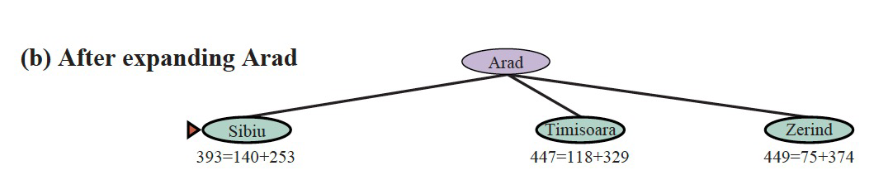
\includegraphics[width=\textwidth]{img/A1.png}
		\end{figure}\begin{figure}[H]
			\centering
			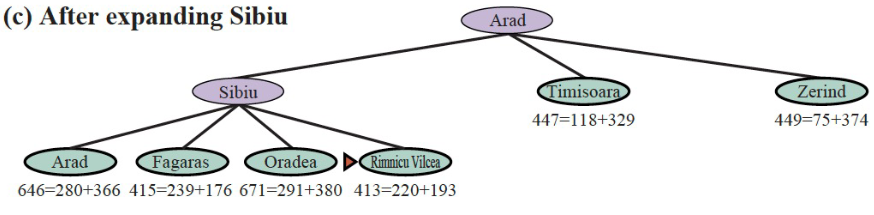
\includegraphics[width=\textwidth]{img/A2.png}
		\end{figure}\begin{figure}[H]
			\centering
			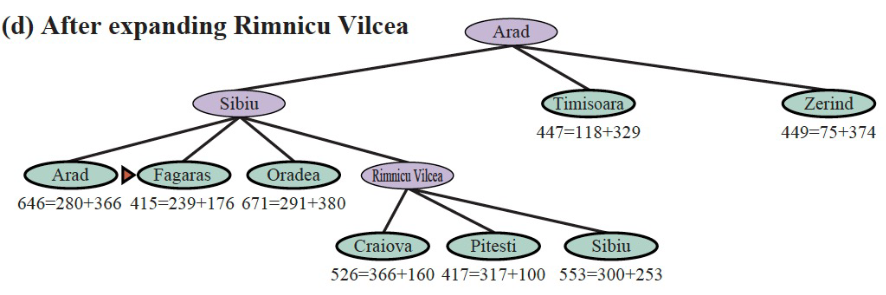
\includegraphics[width=\textwidth]{img/A3.png}
		\end{figure}\begin{figure}[H]
			\centering
			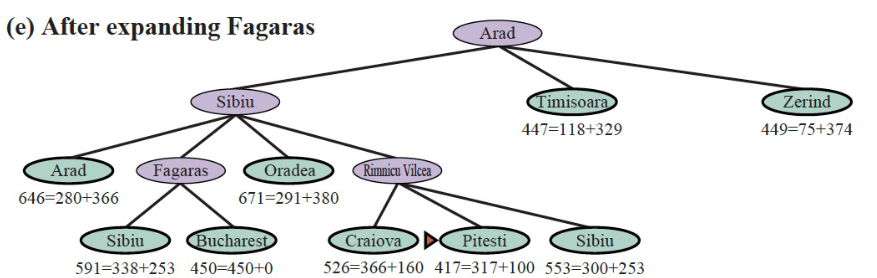
\includegraphics[width=\textwidth]{img/A4.png}
		\end{figure}\begin{figure}[H]
			\centering
			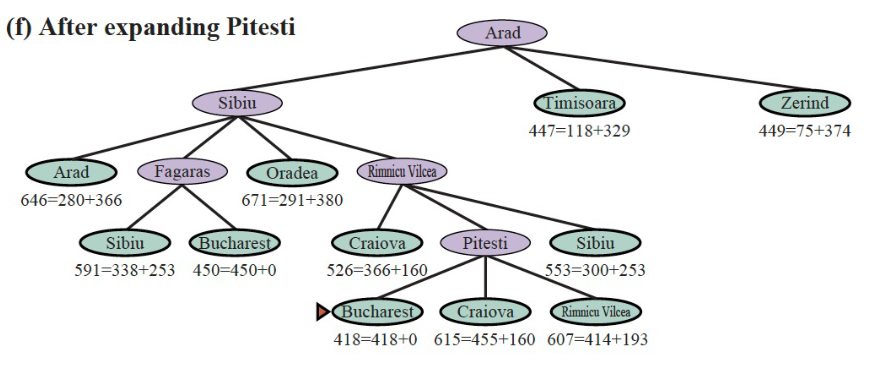
\includegraphics[width=\textwidth]{img/A5.png}
		\end{figure}
		
		\begin{equation}
			f(n) = g(n) + h(n)
		\end{equation}
		
		Avec $g(n)$ le cout du chemin du state initial au node $n$ et $h(n)$ l'heuristique qui approxime le cout du chemin du node $n$ vers le goal.
		
		$g(n)$ est donc un valeur calculé alors que $h(n)$ n'est qu'une approximation.
		
		$h(n)$ ne doit pas surestimer le cout vers le goal
		
		On peut prouver que si A* est optimal si $h(n)$ est admissible.
		
		\textbf{Preuve :}
		\begin{itemize}
			\item Une solutions est chemin initial $\rightarrow$ goal
			\item On pose $C^*$ le chemin a cout minimal
			\item On doit montrer que $A*$ ne retroune pas une chemin suboptimal (une solutions mais pas avec le chemin le plus court)
			\item \textbf{Partie 1}
			\begin{itemize}
				\item $G$ est un goal suboptimal de la frontière
				\item path cost $g(G) = C$ avec $C > C^*$
				\item $h(G) = 0$
				\item $f(G) = g(G) = C > C^* \Leftrightarrow f(G) > C^*$
			\end{itemize}
			\item \textbf{Partie 2}
			\begin{itemize}
				\item $n$ est un node sur le chemin optimal
				\item $f(n) = g(n) + h(n)$
				\item $f(n) \leq C^*$
			\end{itemize}
			\item \textbf{Partie 3}
			\begin{itemize}
				\item $f(n) \leq C^* < f(G)$
				\item Node $G$ ne sera jamais choisis $\Rightarrow$ \textbf{CQFD}
			\end{itemize}
		\end{itemize}
		
			
		Monotonicité de $f(n)$
		\begin{itemize}
			\item Avec $h(n)$ consistent, alors $f(n)$ le long de n'importe quel  chemin est non décroissant (\textbf{Monotonicité})
			\begin{itemize}
				\item On suppose $n'$ successeur de $n$
				\begin{itemize}
					\item $g(n') = g(n) + c(n,a,n')$
					\item $f(n') = g(n') + h(n') = g(n) + c(n,a,n') + h(n')$
					\item Par la consistance, $h(n) \leq c(n,a,n') + h(n')$
					\item $f(n') \geq g(n) + h(n) = f(n)$
					\item $f(n') \geq f(n)$ 
				\end{itemize}
			\end{itemize}
		\end{itemize}
		
		\Large{\textbf{Search Contours}} \normalsize
		
	
			un \textbf{Contour} c'est un groupe de node avec $f(n)$ < une certaine valeur
			
			Le problème de mémoire de A* est a cause que il s'ented de la meme maniere qu'un BFS qui s'etend par courche et A* par f-contours.
			
			\begin{figure}[H]
				\centering
				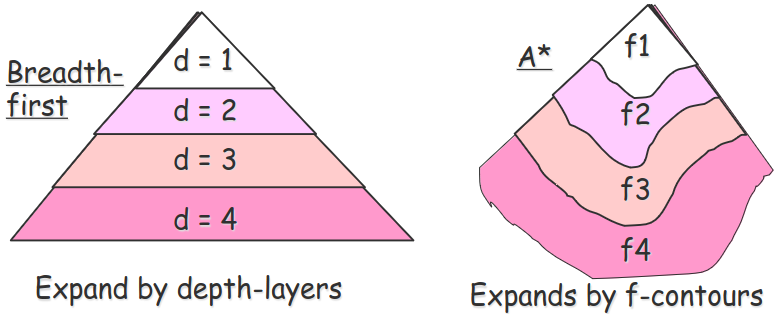
\includegraphics[width=\textwidth]{img/MPA}
			\end{figure}			 
		
			A* étant donc tous les nodes $f(n) < C^*$ et il étand au moins un node du contour $C^*$ avant de trouver le goal.
		
			A* est "optimalement efficace" en utilsnat le graph search car il étend le moins de node
			
			\textbf{Proprités}
			\begin{itemize}
				\item \textbf{Complétude} : Oui
				\item \textbf{Complexité temporelle} : $\mathcal{O}(b^d)$
				\item \textbf{Complexité spatiale} : $\mathcal{O}(b^d)$
				\item \textbf{Optimal} : Oui
			\end{itemize}
			
			Pour réduire le nombre de nodes visité, on peut choisir de pas choisir le node le plus optimal et prendre un suboptimal en utilisant un heuristique pas admissible.
			
			On peut aussi faire en sorte d'utiliser toutes la mémoire disponnible et si on est plein, on décide de retirer les nodes "inutile".
			
		\subsubsection{Weighted A*}
			
			\begin{equation}
				f(n) = g(n) + w.h(n) (\text{avec} w>1)
			\end{equation}
			
			La solution est garantie d'etre dans un interval constant de facteur $w$ de la solution optimal
			
			\begin{center}
			\begin{tabular}{|c|c|c|}
				\hline
				$A*$ & $g(n) + h(n)$ & $w=1$\\ \hline
				Unifirm-cost & $g(n)$ & $w=0$ \\ \hline
				Greedy best-first & $h(n)$ & $w=\infty$ \\ \hline
				Weighted $A*$ & $g(n)+w.h(n)$ & $1<w<\infty$\\ \hline
			\end{tabular}
			\end{center}
			
		\subsubsection{Iterative deepening A*}
			A* avec une limite de depth $l$ qui est incrémenté itérativement.
			
			IDA* expend seulement les nodes avec f-cost() $\leq$ que les nodes non expand a la dernière itérations.
		
			Ce n'est pas efficace quand le nombre des f-cost() sont élevés.
			
			Propriétés :
			\begin{itemize}
				\item \textbf{Complet} : Oui
				\item \textbf{Time complexity} : exponentiel
				\item \textbf{Space complexity} : Linéaire
				\item \textbf{Optimal et $h()$ consistent}
				\item \textbf{Efficace si absence de monotonicité}
			\end{itemize}
			
		\subsubsection{Recursive Best-First Search}		
			DFS combiné avec une meilleur alternative :
			\begin{itemize}
				\item Garde en mémoire les options en marge
				\item Dés que current depth first exploration devient trop couteux, change en
			\end{itemize}
			
		\subsubsection{Simple Memory-Bounded A* (SMA*)}
		
			A* classique et on utilise toutes la mémoire disponible, déq que il y a plus de place, on retire celui avec la pire f-value pour mettre le nouveau
			
			Regénère un arbre de décision seulement quand nécessaire.
			
			\begin{itemize}
				\item \textbf{Complete}: oui si asser de mémoire pour le plus cour chemin
				\item \textbf{Optimal} : Oui si asser de place en mémoire pour stocker le path de la meilleur solutions
				\item \textbf{Complexité temporelle} : Meme que A*
				\item \textbf{Space complexity} : utilise ce qui est disponible

			\end{itemize}
			
			Souvent meilleur que A* et IDA* car bon compromis entre temps et espace
		
	
	\subsection{Heuristic en pratique}
		\subsubsection{Comparer 2 heuristique}	
			On compare le nombre total de node généré N
			
			On compare les arbres de recherches (effective branching factor $b*$)
			\begin{itemize}
				\item On réarrange les arbres en les rendent complet pour les rendre comparables
				\item $b*$ d'un arbre de depth $d$ contient N+1 nodes
			\end{itemize}
			
			Le meilleur heuristique est toujours le mieux informé
			
			$h_2$ sera toujour meilleur que $h_1$ temps que  :
			\begin{itemize}
				\item $\forall \text{node} n : h_2(n) \geq h_1(n)$
				\item $h_2$ domine $h_1$
			\end{itemize}
			
		\subsubsection{Desing d'heuristique admissible}
			Un technique est de simplifier le problème en retirant des restrictions sur les actions.
			
			Le cout de la solutions de ce problème simplifié est toujours une heuristique admissible du probleme original.

\newpage

%Local Search
\section{Local Search}
	On ne s'occupe pas du path dans cette partie, notre but est d'avoir le Goal
	\begin{itemize}
		\item Utilise peut de mémoire
		\item Peut trouver des solution dans une infinité de recherche
		\item Trouve des solutions raisonnable (pas optimal)
	\end{itemize}
	
	On améliore itérativement la solution actuelle. La prochaine solution est dans le voisinage (\textbf{neighborhood}) de la solution actuelle.
	
	\subsection{Optimisation probleme}
		On a une \textbf{Fonction objetive} que on peut maximiser ou minimiser. On veut trouver le Max/Min Global (par ex: distance, nb de queens sur le plateau ...). Le probleme sont les Max/Min locaux et on peut rester coincé dessus.
		
		\begin{figure}[htp]
			\centering
			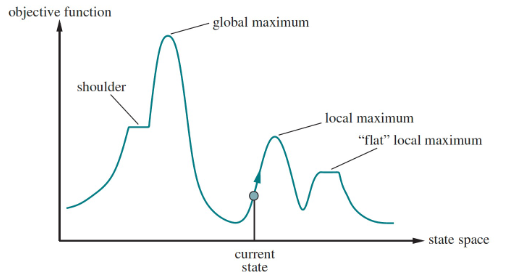
\includegraphics[width=0.5\textwidth]{img/LocalOptiProbleme.png}
		\end{figure}
	\subsection{Neighbourhood}
	
		\textbf{Size}		
	
		Si on décide de choisir un grand \textit{voisinage}, on va avoir des path plus petit pour la solution, mais on va avoir besoin de plus de temps pour parcourir toutes les possibilités. Ils faut trouver un juste milieu entre longueur des paths et temps d'explorations
		
		\textbf{Connectivity}
		
		Pour chaque solution, il y a un path a une solutions optimal. Cela a 2 avantages :
		\begin{itemize}
			\item Pas besoin de recommencer la stratégie (on ne bloque jamais)
			\item Nécessaire pour la propriété de convergence
		\end{itemize}

		\textbf{Contraintes}
		
		Il y a 2 approche possible pour combiner faisabilité avec requièrement optimal
		\begin{itemize}
			 \item Approche 1
			 \begin{itemize}
			 	\item Maintenir la faisabilité à tout moment
			 	\item Explorer seulement les solutions faisable 
			 \end{itemize}
			 \item Approche 2
			 \begin{itemize}
			 	\item Ne pas maintenir la faisabilité à tout moment ;
assouplir un sous-ensemble de contraintes
				\item Explorer un plus grand \textit{Search Space}
				\item Conduire a chercher a des solutions faisable et de qualités
			 \end{itemize}
		\end{itemize}
		
		Un exemple car c'est un peu trop théorique : Graph partitioning
		S
		\begin{figure}[htp]
			\centering
			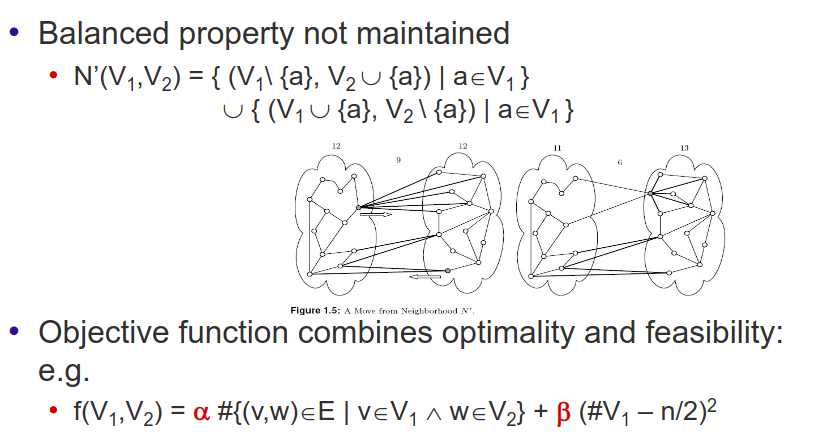
\includegraphics[width=0.7\textwidth]{img/exempleGraphPartionning.png}
		\end{figure}
	\subsection{Heuristic et Metaheuristics}
		\textbf{Heuristics}
		Se concentre sur choisir la prochaine solutions et conduire la recherche avec des optimum local basé sur l'information locale (solutions actuelle et le neighbourhood). utilise peu de mémoire
		
		\textbf{Metaheuristics}
		Tente d'échapper les optimum locaux pour trouver le global optimum basé sur la collecte d'information avec les exécutions faites avants. Prend plus de mémoire car learning derrière.
		
		\textbf{Systematic heuristics}
		Exploration (partiellement possible) du voisinage  pour déterminer solution suivante.
		
	\subsection{Hill Climb Algo}
		\begin{figure}[htp]
			\centering
			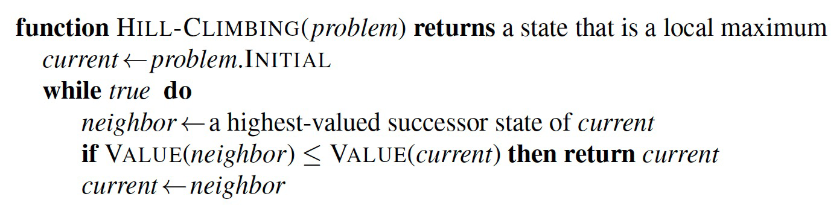
\includegraphics[width=0.7\textwidth]{img/CodeHillClimb.png}
		\end{figure}
		On choisi un state de départ, et on avance dans la direction des valeurs qui augmentes et on stop l'itération quand on ne peut plus aller plus loins. Cette algo va rapidement a la meilleure  solutions mais a plusieurs probleme :
		\begin{itemize}
			\item S'arrête si c'est un Max/Min local
			\item Si on a un plateau, l'algo se stop (on peut mettre un limite d'itération si on tombe la dessus)
			\item Si on a une séquence de Max/Min locaux alors on a du mal a naviguer
		\end{itemize}
		
		Hill climb dépend énormément de la forme du state space et vu que il ne fera jamais de down-hill, si il tombe sur un maxLocal il reste bloqué
		
		\begin{figure}[htp]
			\centering
			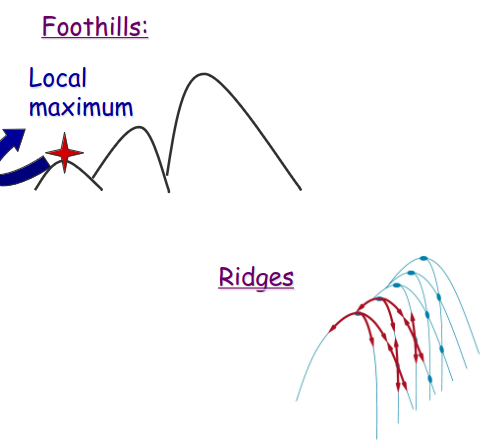
\includegraphics[width=0.6\textwidth]{img/ProblemHillClimb.png}
		\end{figure}			
		
	\subsubsection{Varaintes}
		Il existe plusieures variantes:
		\begin{itemize}
			\item \textbf{Stochastic hill climbing} : Choisis en mode random parmis les mouvements qui monte
			\item \textbf{First-choice hill climbing} : On choisi le premier bon successeur que on trouve, pratique si le nombre de successeur est large
			\item \textbf{Random restart} : On commence de plusieurs points random
		\end{itemize}
	
	\subsection{Random Walk}
		On sélectionne en mode random un élément du neighbourhood et on décide si on doit l'accepter comme la prochaine solution. Il y a plusieur approche possible :
		\begin{itemize}
			\item Amélioration aléatoire
			\item Heuristique de Metropolis : accepter de dégrader la solution
		\end{itemize}
		
	\subsection{Simulated annealing}
		Algo qui combine Hill climb, un scheduler et un metropolis step.
		\begin{itemize}
			\item Toujour avance en montant (uphill) si possible
			\item Parfois aller en descendant (downhill) 
		\end{itemize}
		
		On commence avec beaucoup de random et on reduit graduellement l'intensité du random dans l'algo (Annalogie avec la métalirgue qui chauffe du fer et le laisse refroidir lentement)
		
		Opérations :
		\begin{enumerate}
			\item Toujours aller uphill si possible
			\item parfois (random) aller downhill (quand la témpérature est haute faut laisser redescendre)
			\item C'est assurée d'etre optimal si réduction lente.
		\end{enumerate}
				
	\subsection{Local Beam Search}
		Mélange de hillclimb et annealing en gardant un seul state en mémoire. L'idée est de :
		\begin{enumerate}
			\item garder $k$ states en mémoire
			\item chaque step, générer tous les successeur des $k$ states
			\item On stop si un state est un goal
			\item Sinon, on sélectionne les $k$ meilleur successeurs de la liste complète de tous les successeurs
		\end{enumerate}
		
		L'algo souffre d'un manque de diversité car les states converges rapidement vers la  régions
		
	\subsection{Genetic Algorithms (GAs)}
		Basée sur la théorie de l'évolution (woké en panique). On commence avec $k$ supposition de début (populations), chaque individus  de la population a un string de longueur fixe qui représente son gêne. On produit la prochaine génération en \textbf{reproduisant} les individus de la populations en ajoutants quelque random mutations. Chaque individus possèdes un score de fitness
		
		\begin{figure}[H]
			\centering
			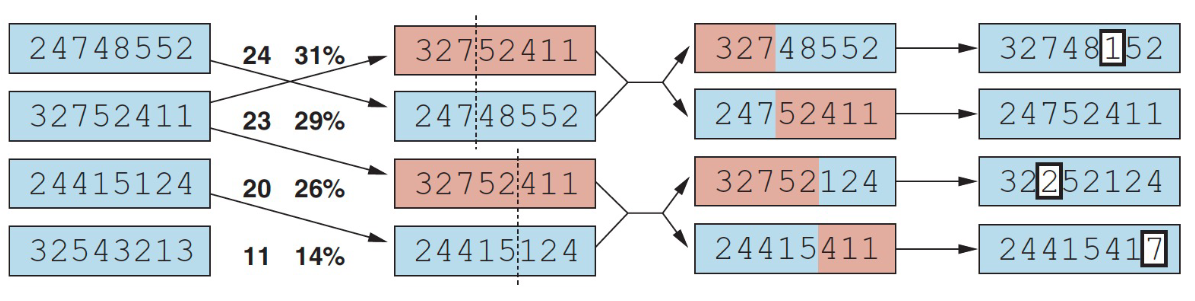
\includegraphics[width=0.7\textwidth]{img/GA}
		\end{figure}
	
		Exemple 8-queens:
		\begin{figure}[htp]
			\centering
			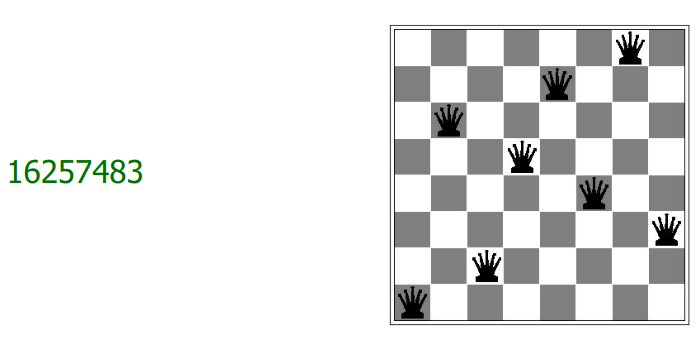
\includegraphics[width=0.5\textwidth]{img/8QueenGA1.png}
			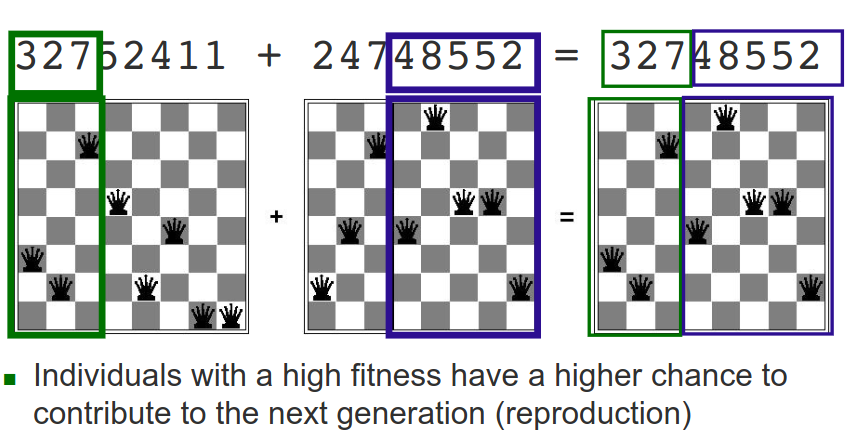
\includegraphics[width=0.7\textwidth]{img/8QueenGA2.png}
		\end{figure}
		
		Les mutations randoms peuvent amener a un bonne situation et permet d'explorer de nouvelle partie du search space
		
		\begin{figure}[htp]
			\centering
			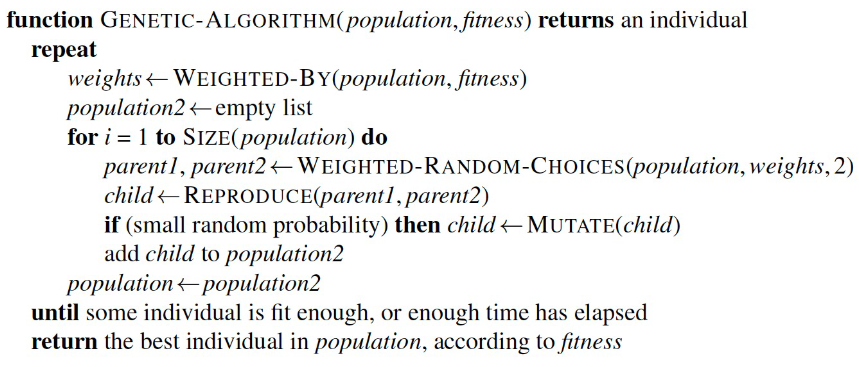
\includegraphics[width=0.7\textwidth]{img/AlgoGA1.png}
			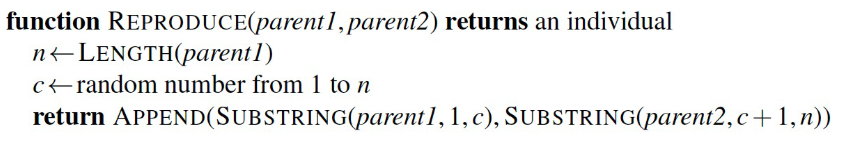
\includegraphics[width=0.7\textwidth]{img/AlgoGA2.png}
		\end{figure}
		
		un probleme avec cet algo est que le crossover est pas applicable a tous les problèmes.
		
	\subsection{Tabu search Metaheuristics}
		
		Sélectionne le meilleur voisin \textbf{qui a pas encore été visité}. Un problème est que c'est difficile de garder la trace de tous les nodes déja visités. Un solutions est de garder en mémoire un suffix de la séquence de node visité.
		
	\subsection{Intensification vs. Diversification}
		\begin{tabular}{|l|p{0.45\textwidth}|p{0.45\textwidth}|}
			\hline
			& Intensification & Diversification\\
			\hline
			\textbf{Goal} & Accroître la recherche dans les domaines prometteurs & Explorer de nouveaux endroit\\
			\hline
			\textbf{Risk} & Convergence prématurée (Max/Min Local) & Convergence vers l'optimal peut prendre du temps\\
			\hline
			\textbf{Mean} & Favorise les bonne solutions & Choix probabiliste des solutions\\
			\hline
			
		\end{tabular}
		
	\subsection{Other Local Search}
		\begin{itemize}
			\item \textbf{Variable Neighborhood Search}
			\item \textbf{Guided Local Search}
			\item \textbf{Adaptive Local Search}
			\item \textbf{Ant Colony Optimization}
			\item \textbf{Statistic Local Search} \footnote{voir slides}
		\end{itemize}
		
	\newpage

\newpage

\section{Constraint Satisfaction Problem (CSP)}

	Le but est de crée un algo de recherche indépendant du type de probleme

	On définit le probleme en 3 composant : 
	\begin{itemize}
		\item \textbf{X} : ensemble des variables $X_1,X_2,...,X_n$
		\item \textbf{D} : ensemble des domaines $D_1,D_2,...,D_n$, un pour chaque variables
		\item \textbf{C} : ensemble des contraintes qui spécifie les combinaison de valeur possible
	\end{itemize}
	
	Les élements de \textbf{C} consiste en une paire $<Scope, rel>$ ou $scope$ est un tuple de toutes les variables impliqué et $rel$ leurs relations
	
	Une solution consiste en une affectation qui ne viole aucune contrainte
	
	Exemple avec les 8-queens car trop dur a comprendre :
		On veut placer 8 reines sur un échequier de sorte a ce que elle ne puisse pas se chevaucher.
		
		On a donc nos variables $X_i$ qui sont les positions (colone) de la reine dans la ligne i $(1 \leq i \leq 8)$\footnote{On sait que il ne peut y avoir que 1 seule reine par ligne et colone car sinon elles se chevauches, on est donc obligé d'utilisé toutes les lignes et colones par une seule reines}
		
		Notre domaine de $X_i$ est alors $\{1,2,3,4,5,6,7,8\}$
		
		Nos contraintes sont que
		\begin{itemize}
			\item 2 reines ne peuvent pas etre sur la meme colone $(X_i \neq X_j)$
			\item 2 reines ne peuvent pas etre sur la meme diagonale $(X_i - X_j \neq i-j) \wedge (X_i - X_j \neq j-i) $
		\end{itemize}
		
		On a donc 8 variables avec 84 contraintes (je vais pas les lister va voir les slides)
		
		
	
	On peut représenté  cela sous la forme d'un graph ou les nodes représente les variables et les edges les contraintes
	
	Il y a différent type de CSP qui dépende du domaine :
	\begin{itemize}
		\item Discret et domaine fini
		\item Discret et domaine infini
		\item Continus et domaine infini
	\end{itemize}
	
	Il y a aussi differente types de contrainte :
	\begin{itemize}
		\item Contrainte Unary : sur seulement une variables (SA $\neq$ Green cf exemple Color mapping Australie slide)
		\item Contrainte binaire : Sur 2 variables ($x+y \leq 12$)
		\item Contrainte High-order : Sur plusieurs variables (peuvent etre transformé en binaire avec des variables additionnel)
	\end{itemize}
		
		Ici on considère seulement les CSP avec contrainte binaire
	
	
	\subsection{Incremental formulation}
		\begin{itemize}
			\item le \textbf{Init state} est une affectation vide
			\item La \textbf{fonction de succession} assigne une valeur a une variable non assignée si aucune contrainte est violé
			\item Le \textbf{Goal test} verifie si l'affectation actuelle est complete
			\item Le \textbf{Path cost} Valeur constante pour chaque etapes qui indique le coup/profondeur du path
		\end{itemize}
			
		Quand une variables est assignié, on propage ça aux autre contrainte et on réduit le search space \footnote{Voire exemple slide 22-27 Chap 5}
		
	\subsection{Forward checking}
		Quand on assigne $v$ à $x$ :
		\begin{itemize}
			\item On vérifie chaque variables non-assignées $y$ connectée a $x$ (par contrainte binaire)
			\item On retire du domaine d'$y$ les valeurs impossible
		\end{itemize}
		
	\subsection{Contrainte de propagation}
			Le but est de réduire le plus possible le search space et trouver un CSP équivalent a l'original mais avec un domaine plus petit
		
			Il y a 2 méthode pour réduire le domaine en considérant les contrainte comme \textbf{Locale}
			\subsubsection{Arc consistency}
			 on considère des contraintes entre 2 variables
			
				$X_i$ est un arc consistant de $X_j$ si pour toutes les valeurs dans $D_j$ il y a une valeur dans $D_j$ qui satisfait la contrainte binaire ($X_i,X_j$)
				\begin{equation}
					X,Y \in \{0,1,...,9\}, X = Y^2 \rightarrow X \in \{0,1,2,3\} \wedge Y \in \{0,1,4,9\}
				\end{equation}
				
				\begin{figure}[H]
					\centering
					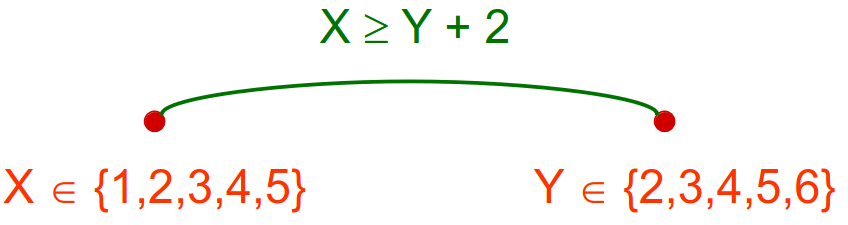
\includegraphics[width=0.7\textwidth]{img/arc.png}
					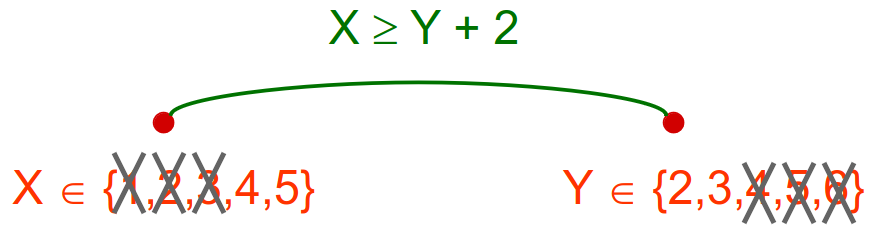
\includegraphics[width=0.7\textwidth]{img/arc1.png}
				\end{figure}
				
				Un contrainte $C(x,y)$ est consistente d'arc si pour toute valeurs dans le domaine de $x$ il y a une valeur dans le domaine d'$y$ qui satisfait $C(x,y)$
				
		\subsubsection{Arc-consistency algorithm}
			\begin{figure}[htp]
				\centering
				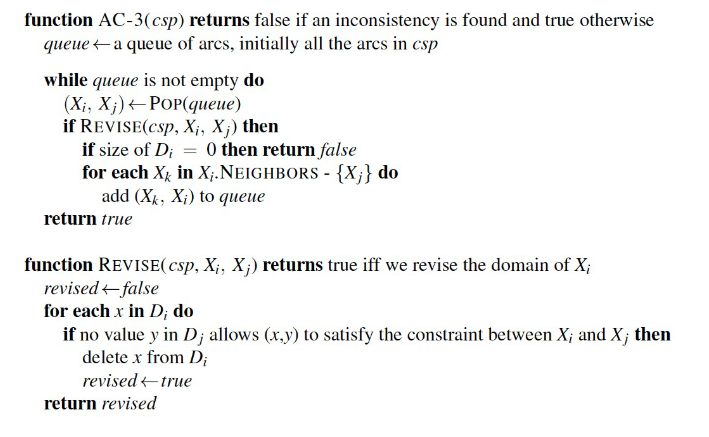
\includegraphics[width=0.7\textwidth]{img/AC-3.png}
			\end{figure}
			
			Avec une complexité de $\mathcal{O}(n^2d^3)$
			
			un peu d'explication :
			\begin{enumerate}
				\item on commence un queue avec un arc initial
				\item temps que il y a $(X_i,X_j)$ dans la queue
				\item si \textit{REVISITE}
				\item alors pour tous les valeurs voisine de $X_i$ sans compter $X_j$, on ajoute $(X_k,X_i)$ dans la queue
			\end{enumerate}
			
			\textit{REVISITE} supprime toutes les valeurs dans $X_i$ tels que elles ne satisfont pas les contrainte entre $X_i$ et $X_j$.


				
		\subsubsection{Bound consistency : }
				Une forme plus faible de \textit{Arc consistency}. On considère seulement les limites du domaine, donc on retire toujours les valeurs sur les limites et jamais au milieu
			
		\subsubsection{Global consistency : }
				Pour les contraintes spéciales, c'est géré avec un "ad hoc specialized method". pour un nombre arbitraire de variable
			
		
			
	\subsection{Backtracking Search for CSPs}
		
			
			L'arbre de recherche a une profondeur de $n$ (nombre de variables) et le nombre de state possible est $\mathcal{O}(d^n)$ avec d la taille du domaine.
			
			La taille de l'arbre est de $\mathcal{O}(n! d^n)$ en raison que le premier niveau est $n.d$ , le deuxieme $(n-1).d$ etc.
			
			CSP seach algo doit seulement considerer une seule variables pour le successeur a chaque node car avec la \textbf{commutativité} quand on assigne une valeur a une variable, nous obtenons la même affectation partielle quel que soit l'ordre
			
		\subsubsection{Backtracking search}
			c'est une recherche par DFS qui choisis une valeur pour une variables et qui reviens en arrière quand une variable plus de valeur qui ne viole pas les contrainte disponibles
		
			\begin{figure}[htp]
				\centering
				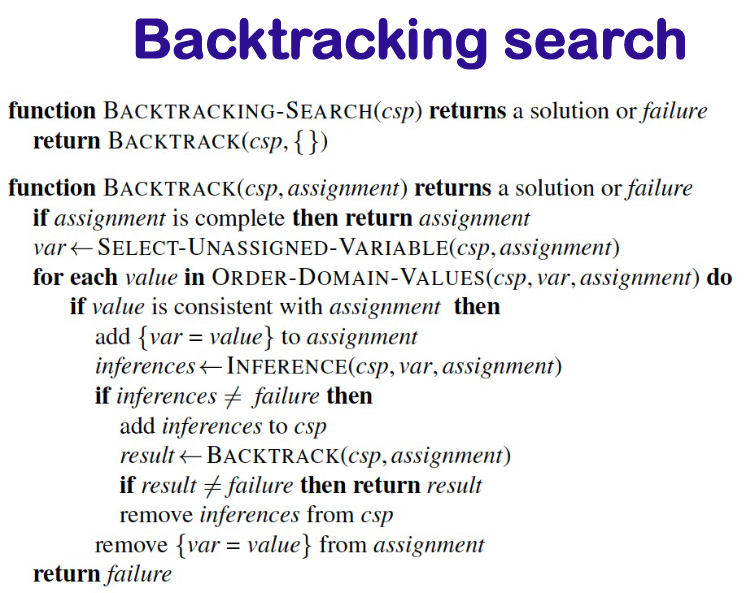
\includegraphics[width=0.7\textwidth]{img/backtrackingSearch.png}

			\end{figure}
			
			\vfill
			
			\begin{figure}[htp]
				\centering
				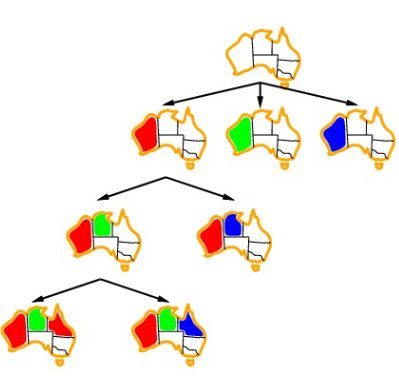
\includegraphics[width=0.5\textwidth]{img/exempleBTS.png}

			\end{figure}
			
		\subsubsection{Variable ordering}
	
			On va optimiser le fait de choisir des variables et des valeurs le tous afin de réduire la recherche
			\begin{itemize}
				\item Minimum Remaining Value (MRV) : on choisis la variable avec le moins de valeur légale
				\item Degree heuristic : on choisis la variables qui entraine le plus grand nombre de contrainte (reduis le facteur de branchement)
			\end{itemize}
			
			\begin{figure}[htp]
				\centering
				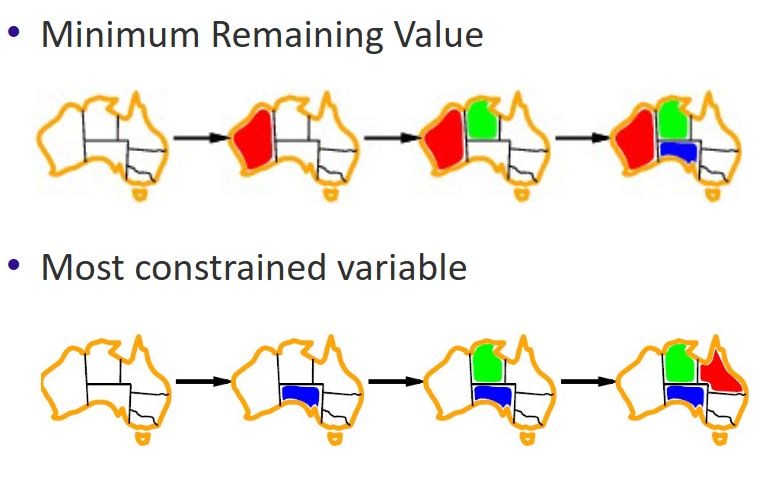
\includegraphics[width=0.5\textwidth]{img/exVarOrd.png}

			\end{figure}
			
		\subsubsection{Interleaving search and inference}
			On veut réduire le \textit{Search Space} pour être plus efficace. Lorsque nous choisissons une valeur pour une variable, nous avons une toute nouvelle possibilité de déduire de nouvelles réductions de domaine sur les variables voisines.
			
			\textbf{Forward checking} : Quand $X$ est attribué a $v$:
			\begin{itemize}
				\item On regarde a chaque variables $T$ non assignées qui sont connectées a $X$
				\item Retirer du domaine $Y$ la valeur incompatible avec la valeur choisie pour $X$.
				
			\end{itemize}
		\subsubsection{Intelligent Backtracking}
			Au lieu de faire un bon en arrière quand on arrive bloquer, on back up a la variables responsable du problème (calculable avec forward checking)
			On garde un \textbf{conflic set} qui garde pour chaque valeur garde l'assignation qui est en conflit avec la valeur.
			
	\subsection{Local Search for CSP}
		\subsubsection{Complete state formulation}
			\begin{itemize}
				\item \textbf{Initial state} : une valeur a chaque variables
				\item \textbf{Sucessor function} : change la valeur d'une variables
				\item \textbf{Goal test} : check si assignement actuelle est consistant et complet
				\item \textbf{Path cost} : Valeur constante par etapes 
			\end{itemize}
			
			Quand on choisie un valeur pour les variables, on choisis avec le minimums de conflit possible
			
		\subsubsection{Min Conflict}
		
			\begin{figure}[htp]
				\centering
				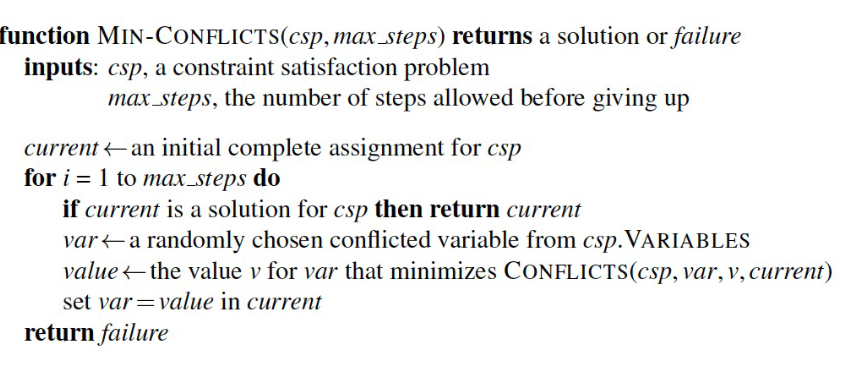
\includegraphics[width=0.8\textwidth]{img/MinConflict.png}
			\end{figure}
			


\newpage

%Adversarial Search and Games
			
\section{Adversarial Search and Games}
	\subsection{Game}
		Un environnement multiagent peut etre vu comme un jeu et donc un problème résolut par recherche.
		Un jeux est défini par :
		\begin{itemize}
			\item \textbf{Initial state} : $S_0$ positions de debut du jeu
			\item \textbf{Player(s)} : quelle joueur a bougé
			\item \textbf{Actions(s)} : ensemble des mouvement légaux qu'il a fait
			\item \textbf{Result(s,a)} : modèle de transition qui définie le résultat du movement
			\item \textbf{Terminal set (s)} : test terminal du state
			\item \textbf{Utility(s,p)} :  valeur numérique du résultat du jeux pour le player $p$
		\end{itemize}
		
	\subsection{MinMax Algo}
	
		\begin{figure}[htp]
			\centering
			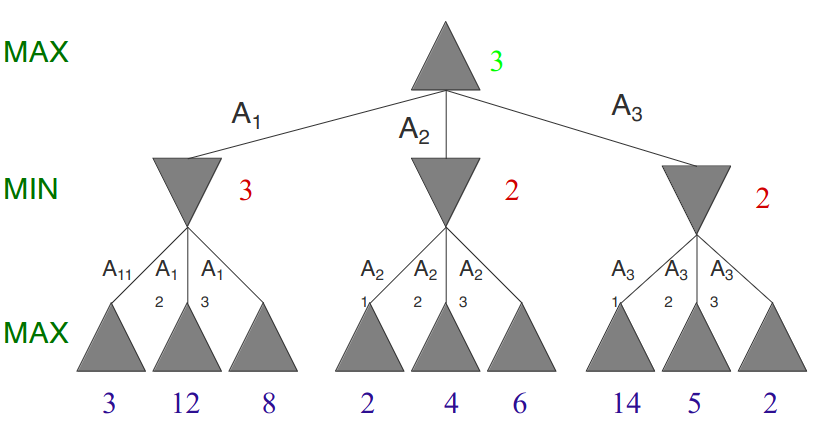
\includegraphics[width=0.7\textwidth]{img/minmax.png}
		\end{figure}
		
		Optimal pour les jeux déterministique et a 2 joueurs. 
		
		Chaque niveau représente a un jourer de jouer en fonction du state, un joueur (MAX) veut maximiser la valeur le deuxieme joueur (MIN) lui veut minimiser
		
		MinMax génère le tree entierement et applique une fonction d'utilité sur les derniers state (les leafs de l'arbre). Ensuite on remontre l'arbre en choissisant le MIN ou le MAX value en fonction du niveau de l'arbre (tours du joueurs). Le node final au dessus représente le meilleur mouvement possible

		\begin{figure}[htp]
			\centering
			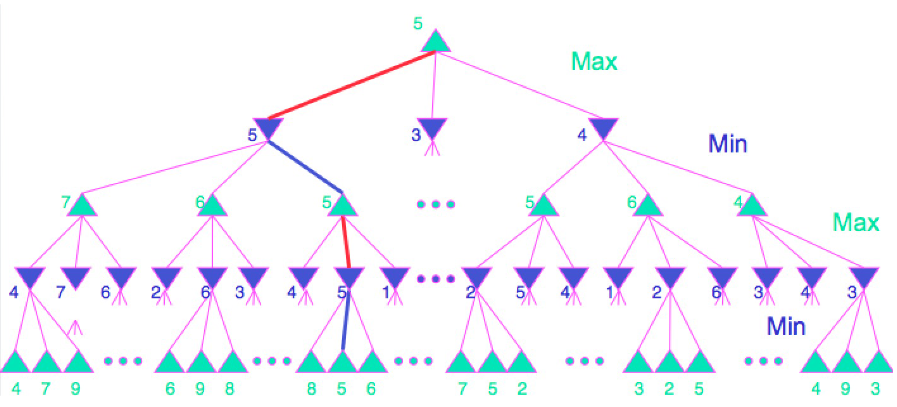
\includegraphics[width=0.7\textwidth]{img/exMinMax.png}
			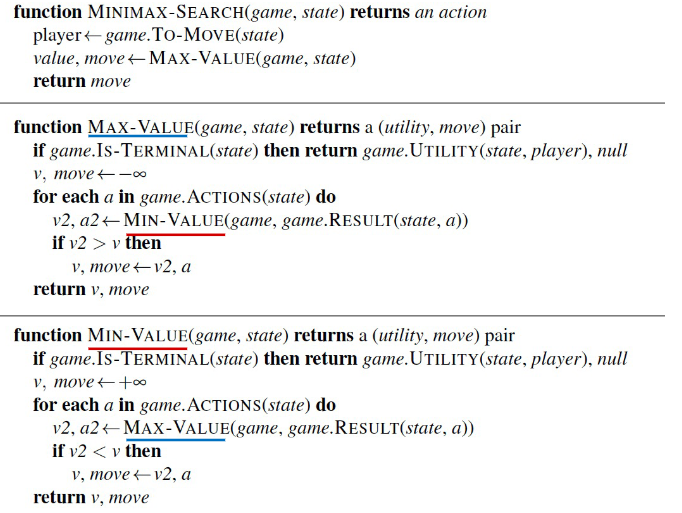
\includegraphics[width=0.7\textwidth]{img/algoMinMax.png}
		\end{figure}
		
		MinMax est basé sur DFS, est complet si le tree est finie. Il a une complexité de $\mathcal{O}(b^m)$ avec $b$ le facteur de branchement et m la profondeur max du tree.
		
		Il est possible de modifer l'algo pour avoir plus de 2 joueurs, il suffit de garder un vecteur a chaque node ou les élements du vecteur sont les utilité de chaque joueurs. Chaque joueur va choisir le mouvement qui maximise l'utilité
		
	\subsection{Alpha-Beta pruning}
		On cherche a "élagué" l'arbre afin de retirer les branche au quelle nous somme sur que il n'y a pas de meilleurs valeurs et donc inutile.Il n'affecte pas le resultat final
		\begin{figure}[htp]
			\centering
			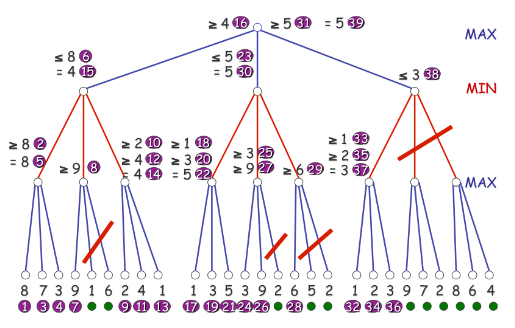
\includegraphics[width=0.7\textwidth]{img/alphabeta.png}
			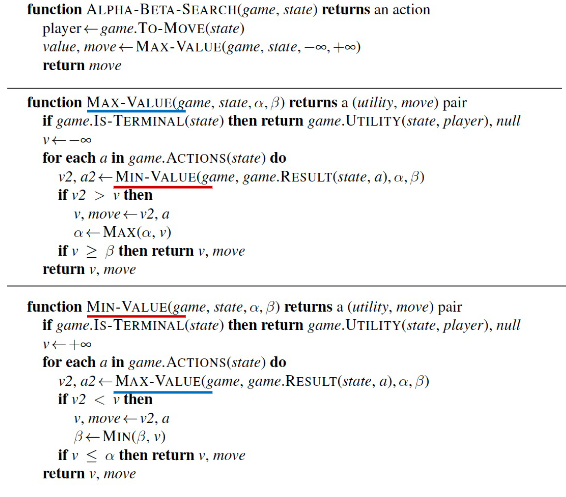
\includegraphics[width=0.7\textwidth]{img/alphabetaalgo.png}
		\end{figure}
		
		$\alpha$ : Valeur du meilleur (plus grande) choix trouvé d'ici la depuis les path visité pour MAX
		
		$\beta$ : Valeur du meilleur (plus petit) choix trouvé d'ici la depuis les path visité pour MIN
		
		Si les sucesseur de l'arbre sont idéalement visité, la complexité temporelle est alors de $\mathcal{O}(b^{d/2})$ et si visité random $\mathcal{O}(b^{3d/4})$
		
		
		\subsubsection{Move ordering}
	
			La disposition des nodes est idéal si le meilleur node est le plus a gauche.
			On peut tenter de réaranger les nodes afin d'avoir les meilleur le plus a gauche, et trouver le \textbf{Killer move}
	\subsection{Imperfect Decisions}
		En pratique il est souvent impossible de faire une research complete car trop grand. Ce que on fait, on fait une search dans seulement un partie du graph. Cela requière a cutoff pour stopper la génération du graph. Mais donc on ne peut pas savoir la valeur, on va donc devoir l'estimer avec une fonction heuristique.
		
		\subsubsection{Evaluation Function}
			La fonction doit etre :
			\begin{itemize}
				\item Consistent avec la fonction d'utilité
				\item équilibré entre présicions et temps de calcul
				\item Dois reflétér la réal chance de gagné
				\item Fonction linéaire avec du poid sont souvent 
			\end{itemize}
			
		\subsubsection{Cutting off the search}
			Approche direct est de stop quand on arrive a une hauteur limite mais il y a un problème si l'état est favorable à un changement rapide dans l'état suivant.
			
			Pour résoudre ce problème, la fonction d'évaluation doit être appliquée uniquement à la position quiescentes, c'est-à-dire stables. (qui ne risquent pas de connaître de fortes variations de valeur dans un avenir proche).			
			
			Il y a \textbf{l'effet d'horizon} : Nous pouvons retarder les catastrophes, mais nous ne pouvons pas les prévenir. Cela peut arriver à cause d'une coupure car l'horizon n'est pas assez profond. Si un agent est confronté à un mouvement qui cause de graves dommages et qui est inévitable à la fin, il essaiera de l'éviter le plus longtemps possible. l'éviter le plus longtemps possible. Au bout du compte, il perdra autant, voire plus.
			
		\subsubsection{Forward pruning}
			Quelques moves a certains nodes sont "élagué" direct sans considérations directed, il coupe les moves "mauvais"
			Avec le \textbf{Beam search}, on considère un ensemble de $n$ mouvement plutot que le tous les mouvements possibles
			
	\subsection{Stochastic Games}
		Ce sont des jeux avec un degré d'improbabilité parmis les elements randoms. Cela requierd une chance pour chaque nodes en plus des Min Max
		
		
		\subsubsection{Expectminimax}
			Cet algo ajoute de la chance aux nodes en plus de MAX MIN. Complexité de $\mathcal{O}(b^{m}n^{m})$ ou $n$ est le nombre de chance d'event distincte

\newpage

%Logical agent
\section{Logical Agent}
	\subsection{Knowledge Based Agents}
		On peut raisoner avec de la connaissance pour savoir quelle action faire. Il y a 2 types de connaissances :
		\begin{enumerate}
			\item \textbf{Logique classique} : Vrai ou fausse
			\item \textbf{Autre logique} : connaissance incertaine
		\end{enumerate}
		
		L'agent peut etre représenté de la sorte : 
		\begin{figure}[htp]
			\centering
			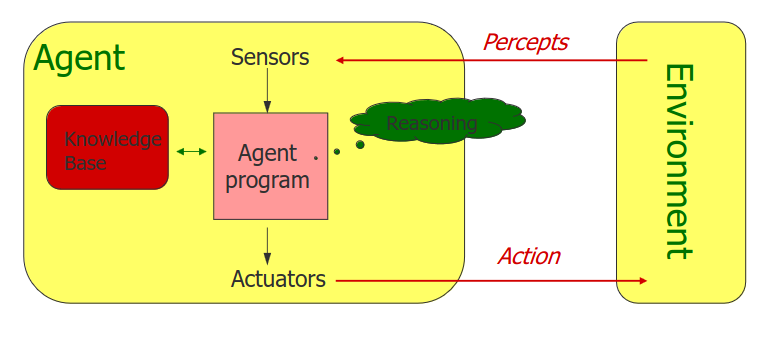
\includegraphics[width=\textwidth]{img/KBA.png}
		\end{figure}
		
		
		Le composant central d'un KBA est un ensemble de phrase (KB).
		
		\textbf{Sentences} : phrase qui est une affirmations sur le monde
			
			
		\subsubsection{Operation KBA}
			\begin{enumerate}
				\item \textbf{TELL :} Ajoute une nouvelle phrase
				\item \textbf{ASK :} Demande se qui est connue
				\item \textbf{MAKE-PERCEPT-SENTENCE} : Construit une phrase affirmant que l'agent a perçu le percept donné à un moment donné.
				\item \textbf{MAKE-ACTION-QUERY} : Construit une phrase qui ASK quelle action devrait etres faite maintenant
				\item \textbf{MAKE-ACTION-SENTENCE} : Construit une phrase affirmant que l'action choisie a été exécutée
			\end{enumerate}
			
			\begin{figure}[htp]
				\centering
				\includegraphics[width=\textwidth]{img/KBA1.png}
			\end{figure}
			
		\subsubsection{Knowledge representation}
			Le language dans laquelle la phrase est représenté. Il y a 2 approches
			\begin{itemize}
				\item \textbf{Declarative approach} : Nous ne disons à l'agent que ce qu'il a besoin de savoir. Les phrases sont dites une à une (par TELL) jusqu'à ce que l'agent sache comment opérer dans son environnement.
				\item \textbf{Procedural approach} : Nous codons les comportements souhaités directement sous forme de programme.
			\end{itemize}
			
	\subsection{Exemple : the Wumpus World}
	
		Une grille avec un créature qui mange les agents. Il y a des puits dans des cases (a éviter) et le but est de trouver le trésor sans se faire manger ni tomber dans les puits.\footnote{pages 209-210-211 du livre}
		\begin{itemize}
			\item Pas entièrement observable (perception local)
			\item Déterministe
			\item Pas épisodique (séquentielle au niveau des actions préformées)
			\item Statique (Monstre et puits ne bouge pas)
			\item Discret
			\item Un seul agent
		\end{itemize}
		
		\begin{figure}[H]
			\centering
			\includegraphics[width=0.8\textwidth]{img/wumpus.png}
		\end{figure}
		
		Avant de faire une action, l'agent dois "réfléchir" a propos de :
		\begin{itemize}
			\item analyser le state actuelle
			\item Eviter les dangers (wumpus et puits)
			\item Trouver le trésor
			\item Garder une version de l'environement (map, propirété des case ...)
		\end{itemize}
		
		\begin{figure}[H]
			\centering
			\includegraphics[width=0.8\textwidth]{img/wumpus1.png}
		\end{figure}
		
		\begin{figure}[H]
			\centering
			\includegraphics[width=0.8\textwidth]{img/wumpus2.png}
		\end{figure}
		
		\begin{figure}[H]
			\centering
			\includegraphics[width=0.8\textwidth]{img/wumpus3.png}
		\end{figure}
	\subsection{Logique}
		
		La logic correspond a de la syntax et de la sémantique
		\begin{itemize}
			\item \textbf{Syntax} : Spécifie toutes les phrases bien formé ($x+y=4$ OK $x2y+=$ KO)
			\item \textbf{Sémantique} : Définir la vérité des phrases par rapport à chaque monde possible
			\begin{itemize}
				\item $x=1, y=3$
				\item $x=2, y=2$
				\item \dots
			\end{itemize}
			\item \textbf{Interprétation} : abstraction mathématique d'un monde possible, en donnant une interprétation une phrase est vrai ou fausse.
			\item \textbf{Modele de phrase} : $\alpha$ est un interprétation ou la phrase est vraie.
			
			"\textit{$m$ est un model de $\alpha$}" $\rightarrow$ $\alpha$ est vrai dans l'interprétation de $m$
			\item \textbf{M($\alpha$)} : ensemble des modeles de $\alpha$
			\item KB $\models$ $\alpha$ : $\alpha$ est vrai si KB est vrai
			\item KB $\vdash$ $\alpha$ : On peut prouver $\alpha$ avec KB 

		\end{itemize}
		
	\subsubsection{Implication (entailment)}
		Implication entre la phrase $\alpha$ et $\beta$, $\beta$ est un conséquence logique de $\alpha$
		
		\begin{equation}
		\alpha \models \beta \ IFF \ M(\alpha) \subset M(\beta)
		\end{equation}
		
		$\beta$ est vrai dans chaque model de $\alpha$ (ex : $x=0 \models xy=0$)
		
		Dans le Wumpus game apres avoir rien détecter en [1,1] et bougé a droite et sentit la brize en [2,1] (signe d'un puit a coté de cette case).
		Toutes les interprétations possible pour KB en assumant seulement des pit est le suivant :
		
		\begin{figure}[H]
			\centering
			\includegraphics[width=0.8\textwidth]{img/modelsWumpus.png}
		\end{figure}
		
		\begin{itemize}
			\item KB = Regles de wumpus + observations
			\item $\alpha_1$ = "[1,2] est safe"
			\item KB $\models \alpha_1$, prouvé par models checking
		\end{itemize}
		
		\begin{figure}[H]
			\centering
			\includegraphics[width=0.8\textwidth]{img/modelsWumpus1.png}
		\end{figure}
		
		\begin{itemize}
			\item KB = Regles de wumpus + observations
			\item $\alpha_2$ = "[2,2] est safe"
			\item KB $\textcolor{red}{\not} \models \alpha_2$
		\end{itemize}
		
		
		si KB $\models$ $\alpha_1$ on peut conclure que $\alpha_1$ est vrai
		
		Verfier KB $\models$ $\alpha$ en utilisant le Model checking
		
		\begin{enumerate}
			\item énumération des interprétations
			\item Trouver les interprétations qui sont un models de $\alpha$
			\item Check que $\beta$ est vrai dans ces models $\alpha \vdash \beta$
		\end{enumerate}
		
		\begin{figure}[htp]	
			\centering
			\includegraphics[width=0.4\textwidth]{img/KBA2.png}
		\end{figure}
		
		\subsubsection{Monotonicité}
			Si KB $\models \alpha$ alors KB $\land \beta \models \alpha$
			
			L'ensemble des formules empliqué ne peut que augmenterau fur et a mesure que des infos sont ajouter au KB
			
			Si une formule est impliquée par un sous ensemble de KB, il est alors aussi impliqué par KB
			
			\begin{figure}[htp]	
			\centering
			\includegraphics[width=\textwidth]{img/process.png}
		\end{figure}
		
	\subsection{Proposition logique}
		\subsubsection{Syntax}
			\begin{itemize}
				\item True, False
				\item Symbols (P,Q,A, \dots)
				\item Connecteur logiques :
				\begin{itemize}
					\item Négations : $\neg$
					\item Conjonctions : $\wedge$
					\item Disjonctions : $\vee$
					\item Implication : $\Rightarrow$
					\item Equivalence : $\Leftrightarrow$
					\item parenthese (,)
				\end{itemize}
			\end{itemize}
			
			\begin{figure}[htp]	
				\centering
				\includegraphics[width=0.6\textwidth]{img/KBA3.png}
			\end{figure}
			
			\subsubsection{Sémantique}
			On fait ça avec un table de verité
			\begin{figure}[H]	
				\centering
				\includegraphics[width=0.6\textwidth]{img/KBA4.png}
			\end{figure}
			
			exemple Wumpus : Un carré est venteux si et seulement si un carré voisins est un puits
			
			$B_{1,1} \Leftrightarrow (P_{1,2} \vee P_{2,1})$
			
			\begin{figure}[htp]	
			\centering
			\includegraphics[width=0.8\textwidth]{img/KB.png}
		\end{figure}			
		\subsubsection{Inference}
			Le but est de decider si KB $\models \alpha$
			
			On veut savoir si $P_{1,2}$ n'est pas un puit :$\neg P_{1,2}$
			\begin{itemize}
				\item Imaginons nous avons ses infos : $B_{1,1}, B_{2,1}, P_{1,1}, P_{1,2}, P_{2,1}, P_{2,2}, P_{3,1}$
				\item on a donc $2^n$ interprétation possible ($n$ = nombre de symbol) donc ici $2^7$
			\end{itemize}
			
			Il faut donc enuméré sur chaque interprétation et check si $\alpha = P_{1,2}$ est True dans chaque models de KB
			
			Complexité temporelle de $\mathcal{O}(2^n)$ et spatiale de $\mathcal{O}(n)$
			
			\begin{figure}[htp]	
				\centering
				\includegraphics[width=0.6\textwidth]{img/KBA5.png}
			\end{figure}
			
	\subsection{Propositional Theorem Proving}
		\begin{itemize}
			\item Equivalence logique : $\alpha \equiv \beta$
			\item Valide (tautologie) : Toutes les intrerprétation sont valide (True)
			\item Satifaisant : True dans certaine interprétation mais pas toutes
			\item Unsatisfait : True pour aucune des interprétations.
			
		\end{itemize}
		
		$\alpha \models \beta IF (\alpha \wedge \neg\beta)$ est insatisfait
			
		\subsubsection{Preuve inference}
			\begin{itemize}
				\item Modus Ponens : $\cfrac{\alpha \Rightarrow \beta, \ \alpha}{\beta}$
				\item And-elimination : $\cfrac{\alpha \wedge \beta}{\alpha}$
				\item Two sens de Morgan : $\cfrac{\neg(\alpha\wedge\beta)}{\neg \alpha \vee \neg \beta} \Leftrightarrow \cfrac{\neg \alpha\vee\neg\beta}{\neg (\alpha \wedge\beta)}$

			\end{itemize}
			
		TODO A TERMINER
		

\newpage

\section{First-Order Logic}
	\subsection{Propositional logic}
		Une proposition logique est :
		\begin{itemize}
			\item \textbf{Déclarative :} les relations entre les variables sont décrites par des phrases
			\item \textbf{Expressive :} peut présenter des informations partielles en utilisant la disjonction
			\item \textbf{Compositionel :} Si $A$ = "il pleut" et $B$ = "j'aime la biere" alors $A \wedge B =$ "il pleut et j'aime la biere"
			\item \textbf{Manque d'expressivité} pour décrire l'environnement de manière concise (ex : ne peut pas dire "les puit provoquent des brises dans les cases adjacentes")
		\end{itemize}
		
		First-Order Logic (FOL) assume que le monde contient :
		\begin{itemize}
			\item Objects : personne, voiture, maison, \dots
			\item Relation : 
			\begin{itemize}
				\item Unary : propriété avec les objets
				\item N-ary : Relations entre les objets
				\item Ex : la relation de fraternité est l'ensemble $(<\text{Bob, Richard}>,<(\text{Richard,Bob})>)$
			\end{itemize}
			\item Fonctions : father\_of, successeur, \dots
		\end{itemize}
	\subsection{Syntax and semantics of FOL}
		\begin{figure}[htp]	
			\centering
			\includegraphics[width=0.6\textwidth]{img/FOL.png}
		\end{figure}
		\begin{itemize}
			\item \textbf{Alphabet :} Variables, constantes; fonctions, \dots
			\item \textbf{Termes :} Combinaison de l'alphabet
			\item \textbf{Formule bien formé} : Construite a partie de symboles de prédicats avec des termes comme arguments et à partir de connecteurs, quantifieurs et ponctuations (selon les regles des connecteurs)
		\end{itemize}
		
		\begin{figure}[htp]	
			\centering
			\includegraphics[width=0.6\textwidth]{img/FOL1.png}
			\includegraphics[width=0.6\textwidth]{img/FOL2.png}

		\end{figure}
		
		quelques exemples :
		\begin{itemize}
			\item Brother(Bob,Richard)
			\item Married(Father(Richard), Mother(Bob))
			\item King(Richard) $\land$ King(Bob)
			\item $\forall x$ King($x$) $\Rightarrow$ Person($x$)
			\item $\exists x$ Crown($x$) $\Rightarrow$ OnHead($x$)
			\item $\forall s$ Breeazy($s$) $\Leftrightarrow$ $\exists r$ Adjacent($r,s$) $\land$ Pit($r$) 
		\end{itemize}
		
		\textbf{Sémantique}
		
			Le domaine de l'interprétation est l'ensembles des objects
			
			\textbf{Constants} : L'interprétation identifies l'object dans le vrai monde.
			
			\textbf{Symbole de prédicats} : L'interprétation spécifie les relation particuliere dans le domaine.Peut etre définie implicitement ou explicitement a travers l'ensemble des tuples d'objets qui satisfait la relations
			
			
			\textbf{Fonctions de symboles} : Identifie l'object référé par un tuple d'objets.Peut etre définie implicitement ou explicitement au travers d'une table.
			
		
		\textbf{Interprétation} : 
		\begin{itemize}
			\item D le domaine
			\item Une fonction (totale) qui map les constantes a D
			\item Une fonction (totale) qui maps les fonctions de symboles as des fonctions ($D \rightarrow D$)
			\item Une fonction (totale) qui maps les symobls prédit a des prédictions ($D \rightarrow Booleans$)
		\end{itemize}
		
		Voire exemple slidesq p18 chap 8
		
		\subsubsection{Complex sentences}
			Elle sont construite en combinant des phrase atomoque en utilisant des connecteurs logique ($\neg, \land, \lor, \Rightarrow, \Leftrightarrow$) et des parentheses.
			\begin{itemize}
				\item $ \neg$ Brother(LeftLeg(Richard), Bob)
				\item Brother(Richard, Bob) $\land$ Brother(Bob, Richard)
				\item \dots
			\end{itemize}
			
		\subsubsection{Quantifiers}
			Peut etre utiliser pour exprimer des propriétés de collections d'objet
			\begin{itemize}
				\item Plus besion d'enuméré chaque objet
				\item $\forall$ dans une conjonction (quantifier universel) ex: $\forall x \ Human(x)\Rightarrow Mortal(x)$
				\item $\exists$ dans une disjonction (quantifier existentiel) ex : $\exists x \ Bird(x) \land Can\_Fly(x)$
			\end{itemize}	
			
			Attention $\forall x \forall y$ est la meme chose que $\forall y \forall x$ pareil pour $\exists$
			
			Mais $\exists x \forall y $ n'est pas la meme chose que $\forall y \exists x$  
			
			$\forall x P$ est pareil que $\neg \exists x \neg P$, pareil pour $\exists x P$ est pareil que $\neg \forall x \neg P$
			
	\subsection{Using FOL}
		\begin{figure}[htp]	
			\centering
			\includegraphics[width=0.6\textwidth]{img/FOL3.png}
		\end{figure}
		
		FOL peut etre utilisé pour modeliser nombre naturel, ensemble de sous ensemble, listes, ...
			
		\subsubsection{Ex Wumpus}
			\begin{figure}[htp]	
				\centering
				\includegraphics[width=0.7\textwidth]{img/FOL4.png}
				\includegraphics[width=0.7\textwidth]{img/FOL5.png}
				\includegraphics[width=0.7\textwidth]{img/FOL6.png}

			\end{figure}
	\subsection{Complement on FOL}
		Voir slides 41-52
		

			


\newpage
\section{Inference in First-Order Logic}
	On va voire comment les algo font pour répondre une question FOL
	\subsection{Propositional vs FOL inference}
		\textbf{Universal Instantiation (UI)} Pour n'importe quelle phrase $\alpha$ , variables $v$, et \textit{ground term} $g$ (terme sans variables)
		
		\begin{equation}
			\cfrac{\forall v \ \alpha}{subst(\{v/g\}, \alpha)}
		\end{equation}
		
		$v$ peut etre remplacer par n'importe quelle instance

		$subst(\omega,\alpha)$ applique la substitution $\omega$ sur $\alpha$
		
		ex : 
		
		$\forall x King(x) \land Greedy(x) \Rightarrow Evil(x)$ Avec on peut déduire que $King(Bob) \land Greedy(Bob) \Rightarrow Evil(Bob)$
		
		\textbf{Existential instantiation}
		Pour n'importe quelle phrase $\alpha$ , variables $v$, et nouveau symbole constant $k$
			\begin{equation}
				\cfrac{\exists \ \alpha}{subst(\{v/k\}, \alpha)}
			\end{equation}
		
		$v$ peut etre remplacé avec un nouveau symbole
		
		ex :
		
		$\exists x  \ mother(bob,x)$ on peut déduire $mother(Bob, ANewMother)$
		
		$ANewMother$ est un constante de Skolem, équivalence déductive (pas d'équivalence logique)
		
		Avec ces deux instantiations, on peut réduire FOL a des symboles de propositions.
		
		\subsubsection{Reduction to Propositional Logic}	
			Le problème est que il y a une infinité de \textit{ground terms} mais grace a Herbrand, on sait que :
			
			\textit{If a sentence $\alpha$ is entailed by a FOL KB, it's entailed by a \textbf{finite} subset of the propositionalized KB}
			
			Application $n=0$ a $\infty$:
			\begin{itemize}
				\item creer un KB propositionnelle en l'instanciant avec un terme de profondeur $n$
				\item regarder si $\alpha$ est entaillé par le KB
			\end{itemize}
			
			Si $\alpha$ est pas entaillé l'algo loop a l'infini
			
			\textbf{Turing} : Entaillement pour FOL est semidécidable
			
	\subsection{Unification}
		C'est une substitution qui fait que des expression logique différente semble identique
		
		ex : 
		
		Parent(Bob,x) et Parent(y,z)
		\begin{itemize}
			\item \{y/Bob, x/z\} : Parent(Bob,z)
			\item \{y/Bob, x/Lucia, z/Lucia\} : Parent(Bob, Lucia)
		\end{itemize}	
		
		L'algo $Unify(p,q)$ prend 2 phrase atomique $p$ et $q$ et retourne une sibstitution qui fait que $p$ et $q$ sont identique.
		
		$Unify(p,q) = \emptyset$ où $Subst(\emptyset, p) = Subst(\emptyset, q)$
		
		$\emptyset$ est l' unificateur des 2 phrases. il y en possiblement plus que 1
		
		\subsubsection{Most General Unifier}
			MGU pour les KOG, fait que "la substitution qui s'engage le moins sur les les variables contraignantes"
			
			ex : 
			
			$Unify(Parent(Bob,x),Parent(y,z)) = \{y/Bob, x/z\}$
			
			MGU est unique
			
		
		\subsubsection{Standardize apart}
			Si 2 phrase partages des variables alors on peut les unifiers, pour eviter les conflits de noms, on renome un des variables.
			
			$Unify(Paren(Bob,x), Parent(y,z)) = Unify(Parent(Bob,w), Parent(q,r))$
		
			\begin{figure}[htp]	
				\centering
				\includegraphics[width=0.7\textwidth]{img/Unification.png}
				\includegraphics[width=0.7\textwidth]{img/Unification1.png}
			\end{figure}
			
		\subsubsection{Generalized Modus Ponens}
			avec $Subst(\emptyset, p_i) = Subst(\emptyset,p_i')$ pour tous les I
			\begin{equation}
				\cfrac{p_1', p_2',\dots,p_n',(p_1 \land,p_2 \land \dots \land p_n \Rightarrow q)}{Subst(\emptyset, q)}
			\end{equation}
			
			ex :
			
			\begin{equation}
			\cfrac{King(Bob), Greedy(y), (King(x) \land Greedy(y) \Rightarrow Evil(x))}{Evil(Bob)}
			\end{equation}
			Avec $\emptyset = \{x/Bob, y/Bob\}$	
			
	\subsection{Forward Chaining}z
		\subsubsection{First-order definite clauses}

		\begin{itemize}
			\item Trouver toutes les regles dont les prémisses sont satisfaites
			\item Ajouter leurs conclusions au faits connus
			\item Repréter l'opération jusqu'a ce qu'une réponse soit apportée a la question  ou qu'aucun fait nouveau n'est ajouté
			
		\end{itemize}	
		
		\begin{figure}[htp]	
			\centering
			\includegraphics[width=0.7\textwidth]{img/ForwardChaining.png}
		\end{figure}		
		
		\subsubsection{Analyse}
			\textbf{Soundness :} Il ne dérive que les phrases qui sont impliquées, parce que Generalize Modus Ponen le fait.
			
			\textbf{Completeness :} Il répond à toutes les requêtes dont les réponses sont impliquées par le KB, mais peut ne pas se terminer en raison de la semi-décidabilité de l'implication avec des clauses définies.
			
	\subsection{Backward chaining}
		Commence  avec les prémisses de l'objectif
		\begin{itemize}
			\item Chaque prémisses doit etre supporté par le KB
			\item Commencer avec la premieres hypotheses et chercher soutient du KB
			
		\end{itemize}
		
		La fonctions est un algo récursive tel que une depth-first.
		
		\begin{figure}[htp]	
			\centering
			\includegraphics[width=0.7\textwidth]{img/BackWardChaining.png}
		\end{figure}		
		
		\subsubsection{Logic programming: Prolog}
			Algorithm = Logic + Control
			
			TODO
			
	\subsection{Résolutions}
		Chaque phrase d'un FOL peut etre convertit en CNF (conjuctive Normal Form)
			
		\begin{enumerate}
			\item \textbf{Eliminer Implications} : $p \Rightarrow q$ devient $\neg  \lor q$ 
			\item \textbf{Bouger  les $\neg$ qui sont devant}  :
			\begin{itemize}
				\item $\neg(p\lor q)$ devient $\neg p \land \neg q$
				\item $\neg(p\land q)$ devient $\neg p \lor \neg q$
				\item $\neg \forall x, p$ devient $ \exists x \ \neg p$
				\item $\neg \exists x, p$ devient $\forall x\  \neg p$
				\item $\neg \neg p$ devient $p$
			\end{itemize}
			\item \textbf{standardiser les variables} : $(\forall x P(x)) \lor (\exists x \ Q(x))$ devient $(\forall x P(x)) \lor (\exists y \ Q(y))$
			\item \textbf{Bouger les quantifiers a gauche} : $p \lor \forall x \ q$ devient $\forall x \ p \lor q$
			\item \textbf{Skolemization} : Voire prochaine sections
			\item \textbf{De Morgan}
		\end{enumerate}
		
		\subsubsection{Skilemization}
			Objectif est de:
			\begin{itemize}
				\item retirer tous les quantifiers existants
				\item Replacer les varaibles par des toutes nouvelles constantes qui n'existe pas de le KB
			\end{itemize}			 
			
			ex : $\exists x \ Q(x)$ devient $Q(A)$ avec où $A$ est unique
			
			Pour les phrases plus complexe, on utilise des fonctions de symbole (Skolem functions) pour indiquer des valeur  spécifique.
			
			ex : $\forall Animal(x,A)$ devient $\forall Animal(x,F(x))$
			
		\subsubsection{Resolution inference rule}
			Pour $p_i$ and $q_i$ où $UNIFY(p_j, \neg q_k) = \emptyset$
			\begin{equation}
				\cfrac{p_1 \lor \dots p_j \dots \lor p_m, q_1 \lor \dots p_k \dots \lor q_n}{SUBST(\emptyset,(p_1 \lor \dots p_{j-1} \lor p_{j+1} \dots \lor p_m \lor q_1 \lor \dots q_{k-1} \lor q_{k+1} \dots \lor q_n))}
			\end{equation}
			
			exemple plus concret :
			
			\begin{figure}[htp]	
				\centering
				\includegraphics[width=0.5\textwidth]{img/RIR.png}
			\end{figure}	
			
			$\alpha$ est un conséquence logique de KB si KB $\models \alpha$ IFF ($KB \land \neg \alpha$) insatisfait
			
			On transforme juste $\neg \alpha$ en CNF et montre que $KB \land \alpha$ insatisfait car apres application des règles de résolutions.
			
			\begin{figure}[htp]	
				\centering
				\includegraphics[width=0.9\textwidth]{img/RIR1.png}
			\end{figure}
			
		\subsubsection{Introducing answers}
		
			\begin{figure}[htp]	
				\centering
				\includegraphics[width=0.8\textwidth]{img/RIR2.png}
			\end{figure}
			
			
\newpage
\section{Automated Planning}
	\subsection{Definition of classical planning}
		Trouver une séquence d'action pour accomplir l'objectif, c'est une combinaison de différentes technique de IA:
		\begin{itemize}
			\item Seaching (Uninformed et informed)
			\item CSP
			\item Prositional logic
			\begin{itemize}
				\item Modélisation
				\item Inference (SAT)
			\end{itemize}
			\item FOL
			\begin{itemize}
				\item modelisation
			\end{itemize}
		\end{itemize}
		
		L'environnement est :
		\begin{itemize}
			\item Entierement observable
			\item déterministe 
			\item fini
			\item statique
			\item discret
		\end{itemize}
		
		C'est similaire a un \textit{Search problem} :
		\begin{itemize}
			\item Input :
			\begin{itemize}
				\item Ensemble de state
				\item Action (State -> State)
				\item Initial state
				\item Goal (1 ou un ensemble de state)
			\end{itemize}
			\item Output
				\begin{itemize}
					\item Séquence d'actions
				\end{itemize}
				
			\item Difficulté : 
				\begin{itemize}
					\item Taille de l'espace de recherche
					\item Methode de recherche
					\item Introduire décoposition du probleme
				\end{itemize}
		\end{itemize}
		
		\subsubsection{Représentation du State}
			C'est un conjonction de (Grand et function free) atoms ($\{A,B\} = A\land B$)
			\begin{equation}
				At(Plane1, Melbourne) \land In(Plane1, Bob)
			\end{equation}
			
			\textbf{\textit{Closes-World Assumption}} : si pas d'information sur $p(a)$ alors $p(a) = False$
			
		\subsubsection{Représentation des Actions}
			Spécifiés avec une \textbf{signature} (noms et paramètres), \textbf{Préconditions} (conjunction of literals), \textbf{Effets} (conjunction of literals)
			
			Une action est \textbf{Applicable} dans une state $s$ si et seulement si le préconditions de $a$ est une conséquence logique de $s$ si et seulement si $s$ satisafait les préconditions de $a$
			
		\subsubsection{Représentation des objectifs}
			Une objectif = une state partiellement spécifié
			
			C'est comme une précondition : une conjonction de litérals (+ ou -)
			
			Un state satisfait un Goal si il contient tous les atoms du goals
		
			
			\begin{figure}[htp]	
				\centering
				\includegraphics[width=0.8\textwidth]{img/BLOCK.png}
				\includegraphics[width=0.8\textwidth]{img/BLOCK1.png}
			\end{figure}
			 \newpage
			
	\subsection{Algorithms for classical planning}
		\subsubsection{Complexité}
			\textbf{PlanSAT} : Demande si il existe un plan qui résoud le planning probleme
			
			\textbf{Bounded PlanSAT} : Demande si il existe une solutions de longueur $k$ ou moins
			
			Les 2 problemes sont décidable (nombre fini de state)
			
			Les 2 problemes sont dans \textbf{PSPACE} (plus difficile que NP) mais pas dans NP, PlanSAT est dans P, Bounded PlanSAT est dans NP-Complet.
			
		\subsubsection{Forward and backward search}
			c'est possible d'utiliser \textit{classical state-space search methods} et avec préconditions/effetst, il es possible de rechercher dans n'importe quelle directions
			
			\begin{figure}[htp]	
				\centering
				\includegraphics[width=0.8\textwidth]{img/FBSearch.png}
			\end{figure}
			
		\subsubsection{Forward state-space search}
			Similaire a la Search Methode (Ch. 3)
			
			Explore pas mal d'actions inutile, de plus state space est tres large(branching factor) c'est pour ca que une fonction heuristique précises est tres utile
			
		\subsubsection{Backward state-space Search}
			On commence du goal et on applique des actions a l'envers jusqu'a trouver une séquence d'etapes qui arrive au state initial. Marche seulement comment on sait faire une actions a l'envers pas toujours le cas. Dure de trouver un bon heuristique.
			
		\subsubsection{Planning as Boolean satisfiability}
			Planning par tester la satisfesabilité le phrase propositionnel $InitialState \land AllPossibleActionDescription \land Goal$
			
			A TERMINER
			
	\subsection{Heuristics for planning}
	
		Recherche forward ou backward est inutile sans un bon heuristique
		
		On cherche a approximer le nombre d'action pour arriver a l'objectif depuis un state donnée
		
		\subsubsection{Relaxed problem}
			On defini un nouveau probleme qui est plus facile a résoudre que le probleme initial, le cout de la solutions de ce probleme devient l'heuristique du probleme initial. On peut par exemple ignorer préconditions heuristique, 
		
		\subsubsection{Set covering Problem}
		
		On retire toutes les préconditions, et on ignonre les litérals supprimé par actions.
		
		\subsubsection{Restricted precondition}
		On retire seulement quelques literals spécifique dans les préconditions
		
		\subsubsection{Ignore-delete-list heuristic}
		Retirer la liste supprimer de toutes les actions ( supprimer l'action négatifs dans les effet )
		
		\subsubsection{Domain-independent pruning}
		Plusieurs States ne sont juste des variantes d'autre states et donc un peu inutile des les visiter et donc on va élagué certaine branche qui sont symétrique
			
		
			
\section{Learning from exemples}
	\textbf{Learning} : Améliorer la performance des prochaines taches apres avoirs faits des observations. On ne peut pas anticiper toutes les situations possible. Le taches future peuvent changer ...
	
	On se concentre seulement sur les learning problem depuis une collections de input/output, apprendre une fonctions qui prédit l'output pour une nouveau input
	
	\subsection{Feedback}
		3 types de feedback et détermine les 3 types d'apprentissage
		\begin{itemize}
			\item \textbf{Supervised Learning} : l'agent observe les inputs et outputs et apprend une fonctions qui match les inputs et outputs
			\item \textbf{Unsupervised Learning} : l'agent apprend des paternes des inputs meme si aucun output est donnés
			\item \textbf{Reinforcement Learning} : l'agent apprend par une succession de récompese ou de punitions en fonctions des ses actions
			
		\end{itemize}
		
	\subsection{Supervised Learning}
		On donne un ensemble d'entrainemenet $(x_1,y_1), \dots , (x_n, y_n)$
			 où $y_i$ est généra par une $f(x_i)$ inconnues. On découvre une fonction $h$ qui approxime $f$
			
			Pour mesurer la précision de l'hypothèse $h$ on test sur un ensemble de test qui est différent de l'ensemble des test utilsé pour le learning de l'agent.
			Un Hypotheses se généralise bien si elle prédit correctement la valeur de $y$ pour de nouveaux exemple
		\subsubsection{Classification VS. Regression}
			\begin{itemize}
				\item \textbf{Classification} : la valeur de sortie est tirée d'un ensemble fini de valeurs
				\item \textbf{Regression} : L'output est un nombre
			
			\end{itemize}
			
		\subsubsection{Ockam's Razor}
			\begin{figure}[H]
				\centering
				\includegraphics[width=\textwidth]{img/razor.png}
			\end{figure}
			
			On choisis toujours l'hypotheses la plus simple et consistente
			
			On donne plus de priorité aux solutions de degréa 1/2 et moins au plus grand (7/8)
			
			il faut choisir $h*$ qui est le plus problable avec les data donnée
			
			\begin{equation}
				h* = arg \ max_{h\ in H} \ P(h|data)
			\end{equation}
			\begin{equation}
				h* = arg \ max_{h \in H} \ P(data|h).P(h)
			\end{equation}
			
	\subsection{Learning Decision Trees}
		Représente une fonctions qui prend un vecteur de valeur en inputs et retourne une décission (un simple valeur). Il trouve ça décission avec une séquence de teste, car chaque node de l'arbre est un test d'un valeur de l'input et les leaf donne la décision.
		
		\begin{figure}[H]
			\centering
			\includegraphics[width=.8\textwidth]{img/tree.png}
		\end{figure}
		
		\begin{enumerate}
			\item \textit{Alternate} : Seulement Si il y a un restaurant alternatif a coté
			\item \textit{Bar} : Seulement si le restaurant a un bar confortable
			\item \textit{Fri/Sat} : True vendredi et samedis
			\item \textit{Hungry} : Seulement si on a faim
			\item \textit{Patron} : Combien de personne dans le restaurant (None, Some, Full)
			\item \textit{Price} : Fourchette de prix
			\item \textit{Raining} : Si il pleut dehors
			\item \textit{Reservation} : Si on a fait une réservation
			\item \textit{Type} : le type de restaurant (francais, Thaie, italien, Burger)
			\item \textit{WaitEstimate} : Temps d'attente moyen (0, 10, 10-30, 30-60, >60)
		\end{enumerate}
		
		\begin{equation}
			Goal \Leftrightarrow (Path_1 \lor Path_2 \lor \dots \lor Path_n)
		\end{equation}
		
	\subsection{Decision tree from exemple}
	
		Exemple sont des tuples $(X_i, y)$ où $X_i = x_{i1},\dots,x_{in}$ sont les attributs en inputs et $y$ un boolean
		
		\begin{figure}[H]
			\centering
			\includegraphics[width=.8\textwidth]{img/DCFE.png}
		\end{figure}
		
	\subsection{The Decision-Tree-Learning Algorithm}
		On veut le tree le plus petit possible, on peut donc choisir l'attribut le plus important ou alors diviser en sous probleme
		\begin{figure}[H]
			\centering
			\includegraphics[width=.8\textwidth]{img/DTLA.png}
		\end{figure}
		
		Quand on crée un arbre de décission, il y a 4 cas possible :
		\begin{enumerate}
			\item Si tous les exemples sont positif (négatif) alors résultate Yes (No)
			\item Si il y a des positif et négatif, alors choisir le meilleur attribut pour les splits
			
			\item Si il n'y a plus d'exemple qui reste retourner une valeur défault
			\item Si il n'y a plus d'attribut qui reste, mais que les exemples sont positif et négatif, alors les exemple sont incohérents. Return la classification plurielle des exemples restants (vote majoritaire)
		\end{enumerate}
		
		\begin{figure}[H]
			\centering
			\includegraphics[width=.8\textwidth]{img/DTLA1.png}
		\end{figure}
		
	\subsection{Entropy}
		Caclule l'incertitude d'une variable random.
		
		\begin{equation}
			H(V) = \sum_{k}P(v_k)\log_2(\cfrac{1}{P(v_k)}) = -\sum_{k}P(v_k).\log_2(P(v_k))
		\end{equation}
		
		ex: piece non truquée (50/50)
		\begin{equation}
			H(Fair) = -(0.5\log_2(0.5) + 0.5\log_2(0.5)) = 1
		\end{equation}
		ex: piece truquée (99/1)
		\begin{equation} 
			H(Unfaire) = -(0.99\log_2(0.99) + 0.01\log_2(0.01)) = 0.08
		\end{equation}
		
		L'entropie d'un boolean random ave une probabilité de True a $q$ (false = $1-q$)
		
		\begin{equation}
			B(q) = -(q.\log_2(q) + (1-q).\log_2(1-q))
		\end{equation}
		
	\subsection{Leaning Curves}
		On split les exemples en un ensemble de training et test. On apprend des hypotheses et on mesure la précision avec l'ensemble des test.
		
		On commence avec un ensemble l'entrainement de 1 que on augmente au fur et a mesure. On peut remarquer que la précission augmente avec un ensemble de trainning plus large. 
		
	\subsection{Ensemble learning}
	
		Générer une collectino/ensemble d'hypothese et combiner leur prédictions. Cela augmente les performance.
		\subsubsection{Bagging}
			\begin{itemize}
				\item On génere $K$ training set avec $N$ exemple
				\item Produit $K$ décision d'algo
				\item Pour un nouvel input
				\begin{itemize}
					\item Predit $k$ hypothese
					\item vote a la majorité
				\end{itemize}
			\end{itemize}
			
		\subsubsection{Random Forest}
			Produit $k$ décision algo sur l'exemple donnée
			
			ça varie en fonction du choix des attribut
			
			A chaque split on fait une restriction random des choix des attributs
			
		\subsubsection{Bootsing}
			Un set d'entrainement avec des poids, chaque exemple associé a un exemple et donc adapte sa méthode d'apprentisage avec les poids.
			
			Génère au debut une hypothese avec un poid de 1, on agmente le poids des exemples mal classé. 
			
			On stop quand on a $k$ hypotheses et on les utilise pour calculer la prediction
\end{document}